\chapter{Magnetic Reconnection observed by Juno}


\blfootnote{*Parts of this chapter were published in - Sarkango, Y., Slavin, J. A., Jia, X., DiBraccio, G. A., Gershman, D. J., Connerney, J. E. P., Kurth W. S., \& Hospodarsky G. B. (2021). Juno observations of ion‐inertial scale flux ropes in the Jovian magnetotail. Geophysical Research Letters, 48, e2020GL089721}

\section{Introduction}
Magnetic reconnection in the magnetotail results in the formation of helical or loop‐like magnetic structures called plasmoids, which contain strong plasma pressure gradients that maximize along the central axis and balance the magnetic forces directed inward \cite{Hones1984StructureActivity, Kivelson1995ModelsPlasmas, Slavin1989CDAWAssessment}. However, a subset of plasmoids, called ``flux‐ropes'', lack strong pressure gradients in their interior, and the magnetic force of the outer wraps is balanced by the strong axial core field present at their center \cite{Moldwin1991PlasmoidsRopes,Sibeck1984MagnetotailRopes}. Flux ropes in which magnetic stresses are completely self‐balancing are referred to as “force‐free” as $\mathbf{J}\times\mathbf{B}=\nabla p = 0$. These force‐free flux ropes correspond to the minimum energy state for a plasmoid that all such structures will evolve toward with increasing time \cite{Priest2013TheLecture,Taylor1974RelaxationFields}. Plasmoids which lack a core field and possess weak magnetic fields at their center compared to their surroundings are termed ``O‐lines''.

Decades of in situ observations in the terrestrial magnetosphere, together with kinetic simulations \cite{Drake2006ElectronReconnection, Drake2006FormationReconnection}, have revealed that magnetic flux ropes in the night‐side plasma sheet can range in size from order 1 to 10 Earth radii \cite{Ieda1998StatisticalObservations,Slavin1995ISEETopologies} to below the local ion inertial length, which is typically on the order of hundreds of km \cite{Eastwood2016Ion-scaleMMS,Sun2019MMSSheet}. The latter are produced due to simultaneous magnetic reconnection occurring at multiple X‐lines due to the tearing instability acting on a current sheet that has thinned to between the ion‐ and electron‐inertial length scales \cite{Daughton2011RolePlasmas,Drake2006ElectronReconnection,Lapenta2015SecondaryFronts}. A similar dichotomy in flux rope size is seen at Mercury \cite{DiBraccio2015MESSENGERMagnetotail,Slavin2009MESSENGERMagnetosphere,Zhong2019Magnetotail}, whose magnetosphere is closest to that of Earth with tail reconnection being driven by a Dungey‐type \cite{Dungey1961b} magnetic flux transfer cycles, but also possesses differences related to its proximity to the Sun and its lack of an ionosphere. Small‐scale flux ropes play an important role in energizing electrons and ions, which can undergo both, adiabatic acceleration due to the evolving flux rope structure \cite{Drake2006FormationReconnection,Le2012ElectronCoalescence,Zhong2019Magnetotail} and nonadiabatic acceleration due to electromagnetic turbulence \cite{Kronberg2019AccelerationRole}.

Plasmoids and flux ropes have also been observed at Jupiter \cite{Kronberg2007AMagnetosphere,Kronberg2008MassParameters,Russell2000SubstormsTail,Vogt2010a,Vogt2014,Woch2002a}, Saturn \cite{Jackman2011CassiniSaturn}, and Uranus \cite{DiBraccio2019VoyagerUranus}. Especially for Jupiter, Dungey‐cycle reconnection is considered to play a minor role \cite{Cowley2008,McComas2007a} and plasmoid release is facilitated primarily by the centrifugal force associated with mass loading and the energization of fresh plasma. Closed field lines on the Jovian nightside stretch freely, thinning the equatorial current sheet and in the process initiating reconnection and the release of plasmoids down the magnetotail \cite{Cowley2015Down-tailMagnetospheres,Kivelson2005DynamicalMagnetosphere,Vasyliunas1983a}. However, single‐spacecraft measurements cannot provide reliable estimates on the three‐dimensional structures of the Jovian plasmoids. Despite the limitations, it was estimated that plasmoids with diameters between 2 and 20 $R_J$ and cross‐tail width between 40 and 70 $R_J$ \cite{Vogt2014} could only account for a loss of $\sim$30-210 kg/s, which is significantly less than the production at Io, estimated to be between 250 and 1000 kg/s. This discrepancy could be a result of the underestimation of the size of the event \cite{Cowley2015Down-tailMagnetospheres} or indicate a different loss mechanism altogether-either a diffusive ``drizzle'' across weak magnetotail field lines or recurring release of small plasmoids \cite{Bagenal2007ThePoles,Kivelson2005DynamicalMagnetosphere}.

Plasmoids and flux ropes observed so far in the Jovian magnetosphere have been fairly large. The mean duration of the observed plasmoids and flux ropes observed by the Galileo spacecraft at Jupiter was determined by \cite{Vogt2014} to be $6.8$ min and by \cite{Kronberg2008MassParameters} to be between 10 and 20 min (The two studies use different definitions for the duration of a plasmoid event). \cite{Vogt2014} estimated the average diameter of the plasmoid to be $\sim$2.6 $R_J$ (where 1 $R_J =$  71492 km) or $1.85 \times 10^5$ km, though they note that because of single‐point measurement limitations, these plasmoid sizes could be larger. Assuming that the equatorial plasma density at a distance of 90 $R_J$ downtail is $\sim0.01$ cm$^{-3}$ \cite{Bagenal2011b} and that the plasma is made up of mostly S$^{+}$, S$^{++}$, O$^{+}$, and H$^{+}$ ions \cite{Kim2020SurveyObservations}, we can approximate a mass of 16 amu for the average singly charged ion and estimate an ion inertial length ($d_i=c/\omega_{pi}$, where $\omega_{pi}=\sqrt{e^2 Z^2 n_i/\epsilon_0 m_i}$ is the ion plasma frequency) of $\sim$10$^4$ km, which is at least an order of magnitude smaller than the diameter of the plasmoids seen by Galileo. Considering that the Galileo magnetometer had a cadence of a few seconds per vector, it would have been difficult to detect sub-ion scale flux ropes or O‐lines, whose in situ signatures would last only a few seconds.

The dichotomy seen at the other planets and in simulations of reconnecting fields leads to a natural question of whether ion‐scale flux ropes exist in the Jovian magnetotail and if they can be identified using the high‐resolution capabilities of the Juno instrument suite. Recent plasmoid observations by the Juno spacecraft reported by \cite{Vogt2020MagnetotailObservations} have corroborated the Galileo observations, in that large plasmoids lasting several minutes on average were observed. In this work, we extend upon previous Galileo and Juno investigations and present two ion‐inertial scale flux ropes observed by Juno in the dawn‐side Jovian magnetotail, which lasted roughly 22 and 62 s. The local plasma density surrounding these flux ropes is estimated using the low‐frequency cutoff for the continuum radiation as observed by the Juno Waves instrument (e.g., \citeA{Barnhart2009ElectronSpectra}), which shows that these durations correspond to plasmoid diameters comparable to the ion‐inertial length. This study is the first reported observation of magnetic flux ropes on the ion scale in Jupiter's magnetosphere and shows that while reconnection on the global scale at Jupiter's magnetosphere is influenced by the Vasyliunas cycle, as evidenced by the large plasmoids seen by both Galileo and Juno; small‐scale reconnection also occurs and secondary magnetic islands are generated in the Jovian magnetotail, similar to observations at Earth and Mercury. 

\section{Methodology}
We use high‐resolution magnetometer data in the Jupiter De‐Spun Sun (JSS) coordinate system. The Z axis for the JSS system is aligned with Jupiter's north pole, X points toward the sun and Y completes the right‐handed coordinate system. Also used are the corresponding magnetic field components in the spherical polar JSS system ($B_r$, $B_\theta$, $B_\phi$) referring to the radial, co‐latitudinal and azimuthal directions. The Juno Magnetometer investigation measures the magnetic field strength and direction ambient to the spacecraft using boom‐mounted fluxgate magnetometers \cite{Connerney2017TheInvestigation} and measures at rates of 16–64 vectors/second. These high cadence rates are significantly greater than what was returned by the Galileo magnetometer (between 24 and 60 s per vector, e.g., \citeNP{Vogt2010a,Vogt2020MagnetotailObservations}) and they allow us to study smaller scale structures durations down to $\sim$100 ms. We also use data from the Juno Waves instrument \cite{Kurth2017TheInvestigation}, which measures the fluctuations in the electric field between 50 and 40 MHz and in the magnetic field from 50 and 20 kHz. We use the low frequency cutoff for the continuum radiation to infer the electron density \cite{Barnhart2009ElectronSpectra}. 

The magnetic field observations are also supported by plasma observations made by the JEDI energetic particle detector \cite{Mauk2017TheMission}, which measures fluxes of the electrons in the energy range between 25 keV to 1 MeV, protons in the range of 10 keV to 2 MeV and oxygen and sulphur ions in the range of 45 keV to 10 MeV. Three JEDI instruments are located on the Juno spacecraft. Each instrument contains 6 solid-state detectors (SSDs), which measure the flux and can provide an estimate of the particle travel direction. The Juno spacecraft's primary mission was to understand the near-planet polar regions, and hence, JEDI data rates for the outer magnetosphere are lower to accommodate data transfers during this portion of the Juno orbit \cite{Mauk2017TheMission}.  

\begin{figure}
    \centering
    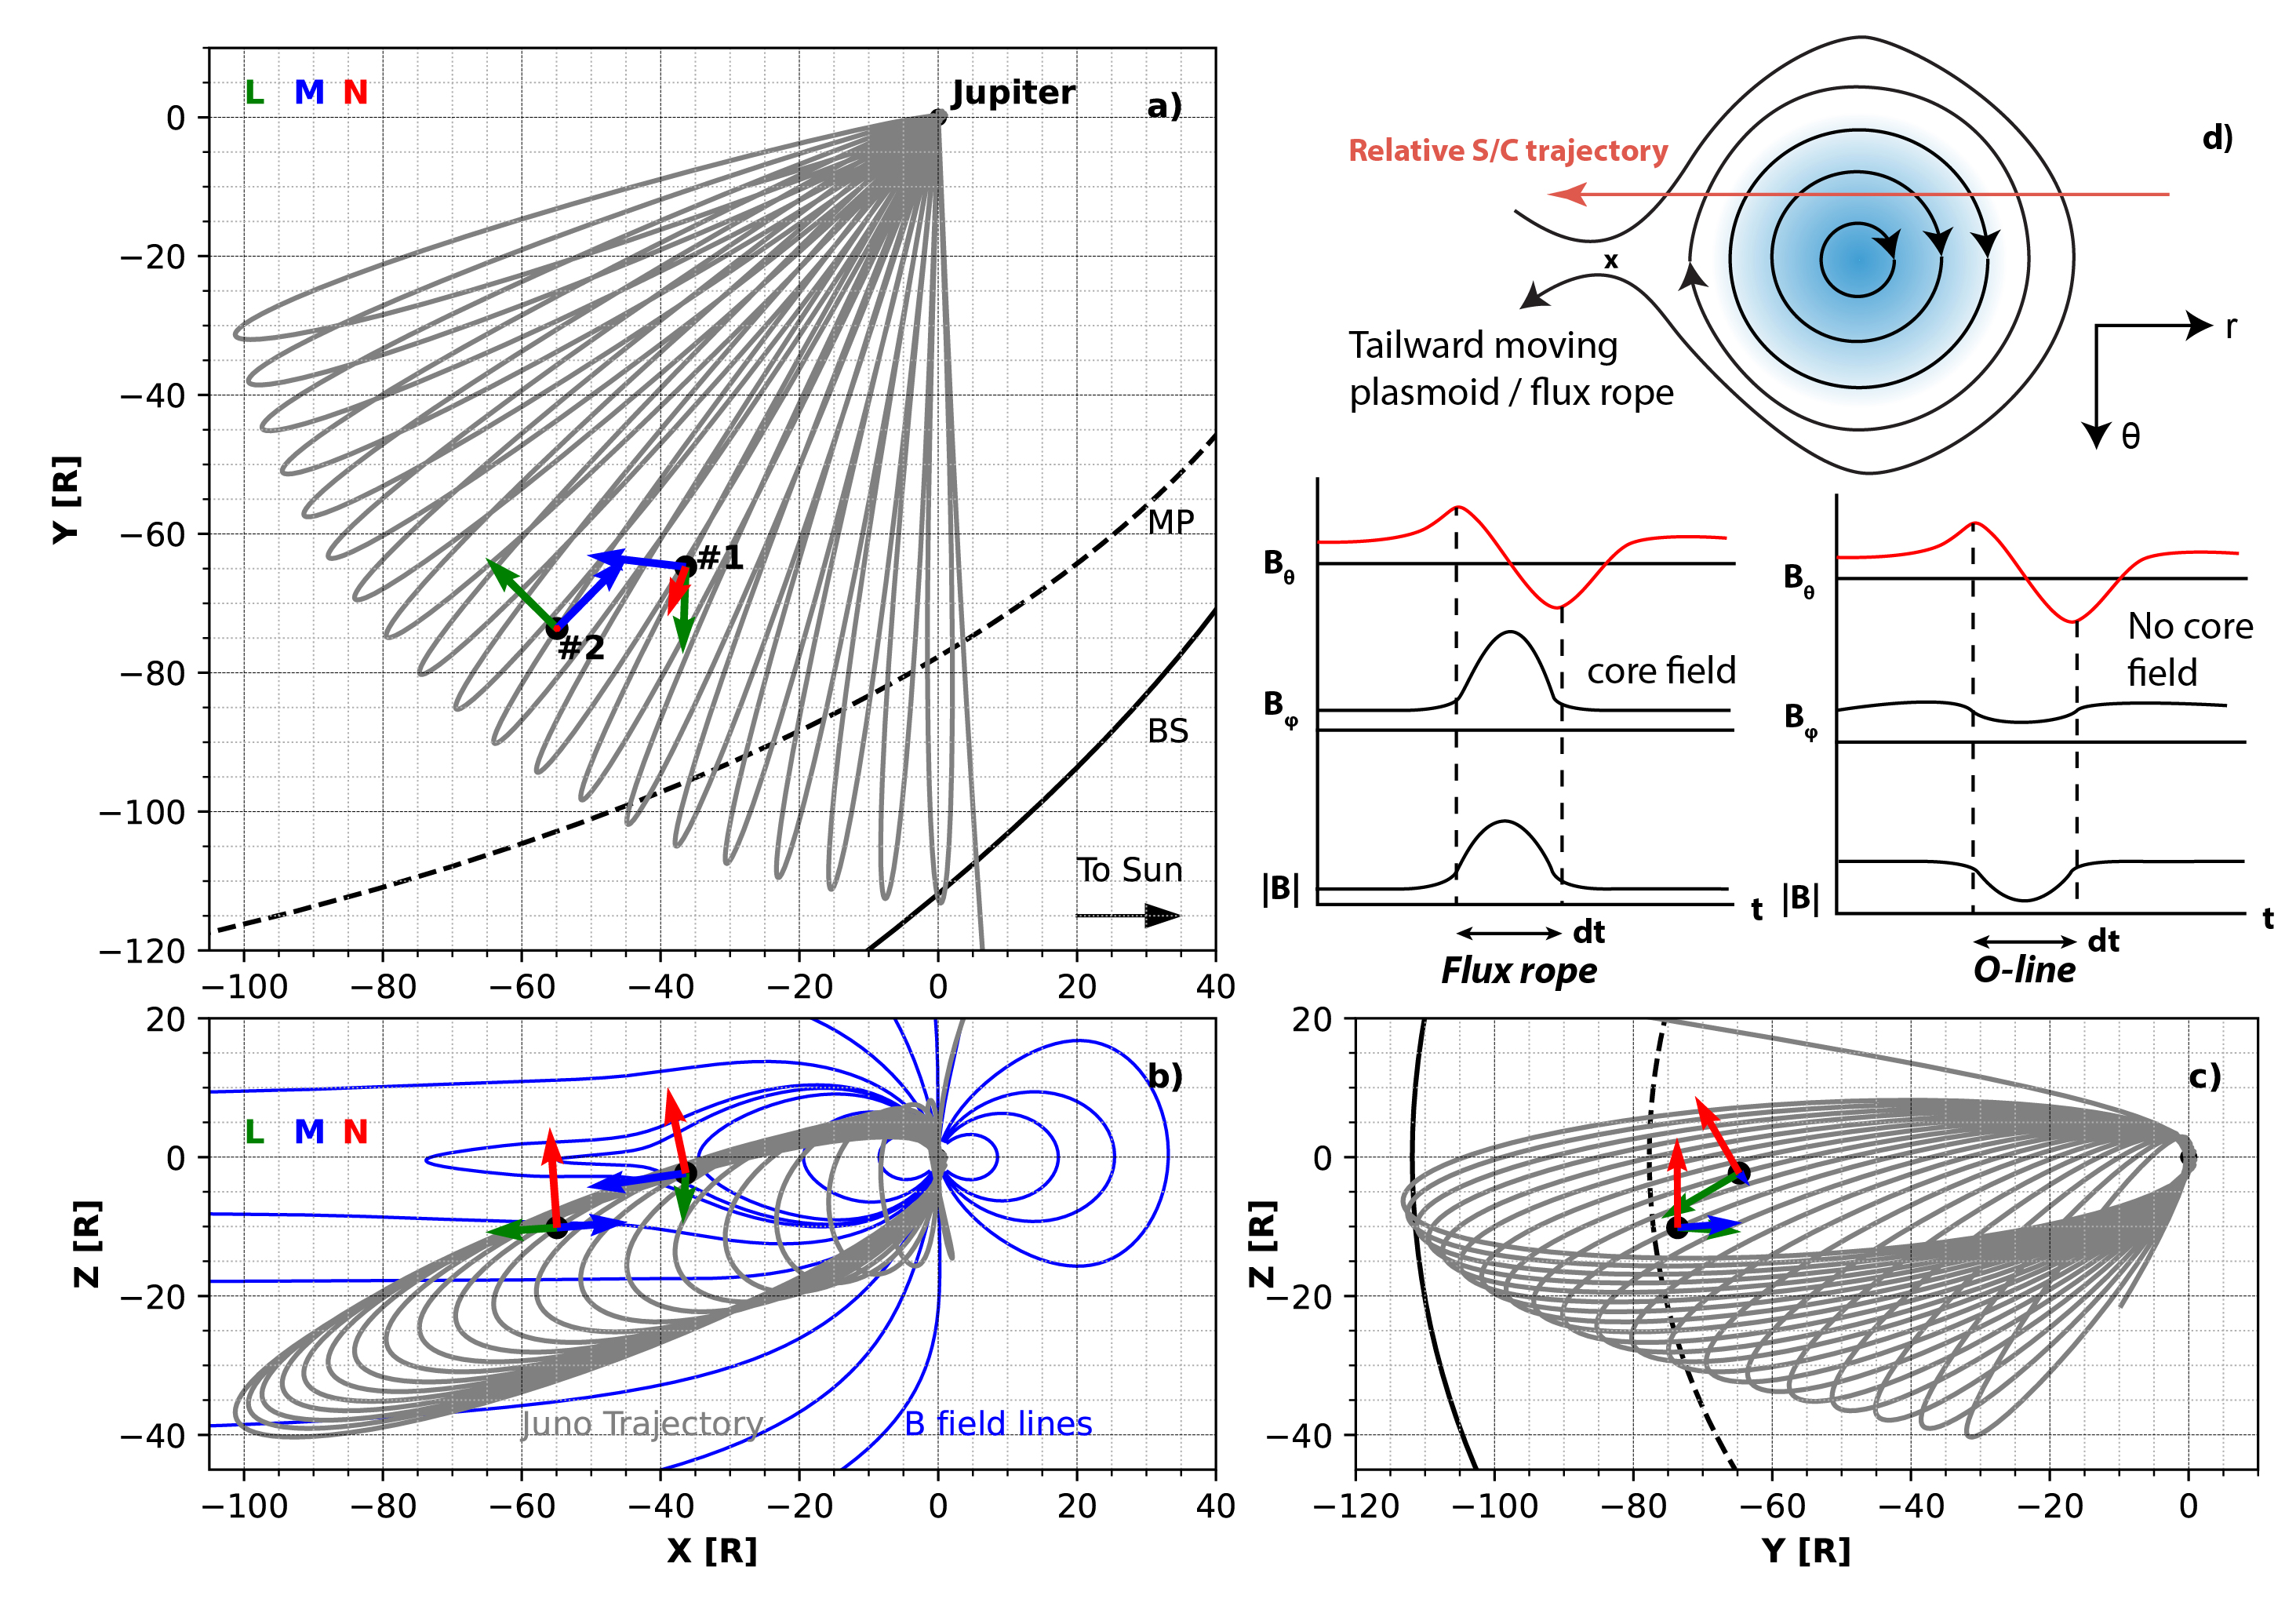
\includegraphics[width=\textwidth]{images5/locations-fluxropes.jpg}
    \caption{The trajectory of the Juno spacecraft in the Jupiter system is shown in panels a, b, and c. Superimposed on panel b are magnetic field lines extracted from the MHD simulation described in previous chapters. The location for two flux rope events are identified and the directions of minimum, intermediate and maximum variance are highlighted via arrows. In panel d), we show the expected magnetic signature of a tailward moving O-line versus a flux rope.}
    \label{fig:locations-fluxropes-eg}
\end{figure}

Juno orbits Jupiter in a highly elliptical trajectory, with each perijove pass separated by $\sim$53 days. However, Juno spent a reasonable amount of time in the equatorial region (Figure \ref{fig:locations-fluxropes-eg}), which enabled it to capture multiple current sheet crossings on every inbound pass. 

In this study, as in \citeA{Vogt2010a,Vogt2014}, positive values of $B_\theta$ indicate a field pointing in the negative $Z_\text{JSS}$ direction at the equator. In the quiet state with Jupiter's magnetic moment pointing north, the equatorial magnetic field is primarily in the positive $B_\theta$ (negative $Z_\text{JSS}$, assuming no current sheet tilt) direction. The magnetic signature of a tailward‐moving plasmoid passing over a spacecraft near the equatorial plane is primarily observed in the $B_\theta$ component as a slight increase and subsequent reversal to negative values (e.g., Figure \ref{fig:locations-fluxropes-eg}d for the signature of a tailward moving plasmoid). As the plasmoid passes over the spacecraft, the return to positive values can either be symmetric, hinting at reconnection occurring in closed field lines, or gradual, indicative of a postplasmoid plasma sheet that is formed when reconnection has progressed to the tail lobes \cite{Jackman2011CassiniSaturn,Jia2012}. Conversely, planetward moving plasmoids would exhibit the opposite signature, that is, an increase of $B_\theta$ in the negative direction and a reversal to positive values. If the plasmoid possesses a core field, it should typically be identified by a peak in the cross‐tail component, either $B_y$ or $B_\phi$ as well as a corresponding peak in the magnetic field strength which roughly matches the time where the reversal in $B_\theta$ is observed. Most plasmoids observed in Jupiter's plasma sheet (e.g., \citeNP{Vogt2014,Vogt2020MagnetotailObservations}) lack an axial core field and are identified as O‐lines. This result is similar to what has been observed at Saturn \cite{Jackman2011CassiniSaturn} and could be due to large plasma pressure in a high $\beta$ plasma and their primary role of carrying plasma away from these planets and balancing the plasma derived from their moons \cite{Cowley2015Down-tailMagnetospheres,Kivelson1995ModelsPlasmas}.

Using the high‐resolution Juno data, we searched for bipolar variations in the $B_\theta$ component in proximity to current sheet crossings to identify flux rope signatures which are roughly 1 min or less in duration. Current sheet crossings (identified by a reversal in $B_r$) are observed only during the planet bound phase of Juno's trajectory with a periodicity of roughly 10 h, which reduces the search duration. As reported by \cite{Vogt2020MagnetotailObservations}, Juno frequently observed bipolar variations close to current sheet crossings. This is more evident in the high‐resolution data and we show two promising examples in this study (Figures 2–4). 

\subsection{Minimum variance analysis}
The minimum variance analysis (MVA) can be used to identify the orientation of a flux rope with respect to the magnetotail \cite{Sonnerup1967MagnetopauseObservations}. For the given time interval, the covariance matrix $\mathbf{M}^{3\times3}$ is first estimated as,

\begin{equation}
    M_{i,j} = \langle B_i B_j \rangle - \langle B_i\rangle \langle B_j\rangle \quad  i,j \in \{x, y, z\}
\end{equation}

The eigenvectors of the covariance matrix, $\mathbf{M}$ ‐ $\mathbf{x}_L$, $\mathbf{x}_M$, and $\mathbf{x}_N$ represent the directions of minimum, intermediate and maximum variance, respectively. For magnetic flux ropes, which possess a helical field on the outside and a unidirectional axial field on the inside, the axial direction can be inferred using the eigenvector of intermediate variance ($\mathbf{x}_M$). There are additional criteria required to identify a flux rope using MVA: A bipolar signature in the maximum ($B_N$) varying component should be present and the eigenvector of the maximum variance should be predominantly in the direction normal to the current sheet. The ratio of maximum to intermediate ($\lambda_N / \lambda_M$) and intermediate to minimum ($\lambda_M / \lambda_L$) eigenvalues must be relatively large (ideally larger than 3 or 4, e.g., \citeNP{Lepping1990MagneticAU}) for the orthogonal coordinate system to be well‐defined. A rotation should be observed in the $B_M$ - $B_N$ hodogram. An almost zero $B_L$ indicates that the spacecraft passed close to the center of the flux rope or O‐line. For a flux rope, the core field should be seen as an enhancement in the $B_M$ component, whereas for an O‐line, a local minimum in the $B_M$ component would be seen. 

Recently, \citeA{RosaOliveira2020NewClouds} have put forward a new metric to verify the degeneracy of the eigensystem using a single parameter $P$ and suggest that $P > 4.5$ is sufficient to verify the consistency of the MVA analysis.

\begin{equation}
    P = 100 \times \frac{\left(\sqrt{\lambda_N} - \sqrt{\lambda_M} \right) \left(\sqrt{\lambda_M} - \sqrt{\lambda_L} \right) \left(\sqrt{\lambda_N} - \sqrt{\lambda_L} \right) }{\sqrt{\lambda_N^3}}
    \label{eqn:mva-p}
\end{equation}

\subsection{Force-free flux rope fitting}
Under the force-free assumption, pressure gradients and the $\mathbf{J}\times\mathbf{B}$ force are considered to be negligible. In this case, the Lundquist solutions can be used to model a circular force-free flux rope \cite{Lepping1990MagneticAU,Slavin2003GeotailSheet} as, 

\begin{align}
    B_A & = B_0 J_0 \left( \alpha r \right)\\
    B_T & = B_0 H J_1 \left( \alpha r \right)
\end{align}

Where $B_A$ and $B_T$ are the axial and tangential field components, $B_0$ is the maximum core field of the flux rope, $\alpha$ is a constant parameter, $r$ is the distance to the center of the flux rope normalized to its radius and $J_0$ and $J_1$ are Bessel functions of the first kind. Since the velocity at which the plasmoid moves cannot be estimated without making assumptions, we cannot estimate the radius of the flux rope directly. Instead, we estimate the impact parameter ($IP$) defined as the ratio of distance to the center of the flux at closest approach to the radius of the flux rope. The parameters $B_0$, $IP$, the flux rope orientation $(\theta_A, \phi_A)$ and the handedness $H$ are varied so as to minimize reduced $\chi^2$ defined as \cite{Lepping1990MagneticAU}

\begin{equation}
    \chi_r^2 = \frac{1}{N} \sum_{i=1}^{N} \left[ \left(B_x - B_{x,m} \right)^2 + \left(B_y - B_{y,m} \right)^2 + \left(B_z - B_{z,m} \right)^2 \right]
\end{equation}

Where $B_m$ is the modeled field and N is the number of data points in the reconstruction. The intermediate direction provided by MVA is used as the initial guess for the orientation of the flux rope  and the minimization is performed in two steps - first using a unit normalized magnetic field with $B_0=1$ nT and then with $B_0$ as a variable parameter to fit the core field strength. A non-linear least squares minimization is used to fit the different parameters \cite{Newville2018Non-LinearPython}. 

\subsection{Automated detection of flux ropes / O-lines}
We use an algorithm which detects possible flux ropes and O-line based on the magnetic field signatures to construct a list of such events and study their properties, such as, frequency and region of occurrence and their duration, which provides an estimate of the size of the plasmoid signature. The algorithm is described below. 

In a given magnetometer data file, which typically contains data for the entire day (UTC), we first identify all times corresponding to a reversal in $B_\theta$, either from positive to negative values or vice versa. Out of the selected crossings, those which occur beyond $r=100 R_J$ and local time less than 05 LT are discarded to prevent contamination due to the magnetopause, where the variability in the magnetic field is quite large. Then, for each $B_\theta$ reversal ($t_\text{0}$), the corresponding start ($t_s$) and stop ($t_e$) times are inferred using the algorithm used by \citeA{Smith2017AutomatedIdentification}. This is achieved by identifying all local extrema in $B_\theta$ near $t_0$ within a particular window size ($\delta t_w$) and finding the maxima-minima (or minima-maxima) pair that when interpolated using a linear function, maximizes the coefficient of determination \cite{Smith2017AutomatedIdentification}.

In order to select changes in the field which are prominent with respect to the background conditions, we discard all those events where the change in $B_\theta$ is less than 2 nT, or less than the standard deviation of the field for a duration of +/- 5 times the window size, i.e. where $\Delta B_\theta = |B_\theta(t_e) - B_\theta(t_s)| < 5\sigma ( B_\theta(\delta t_w))$ or $\Delta B_\theta < 2$ nT. To further improve the quality of selected events, we also discard those times where the excursion in the positive values exceeds that in the negative values by a factor of 2 or more (and vice versa). 

The event list is further refined based on the minimum variance analysis. The unit eigenvector of the variance matrix which provides the direction of maximum change in the field ($\mathbf{x}_N$) must have a $z$-component larger than $0.8$. The ratio of the the eigenvalues corresponding to the minimum, intermediate and maximum directions must be larger than 3, i.e. $\lambda_N / \lambda_M > 3$ and $\lambda_M / \lambda_L > 3$. The $P$ parameter (described by Equation \ref{eqn:mva-p}) must be larger than $4.5$. 

We also specify a condition that the component of the magnetic field showing the least variation ($B_L$) be less than 2 nT, to only capture those events which pass through the center of the plasmoid structure. Similarly, we place a similar limit on $B_r$, which should be less than 3 nT, to prevent contamination due to any process in the magnetotail lobes. The latter condition implies that we only identify events which occur close to the magnetotail current sheet.



\section{Results - Case studies}
\subsection{Event 1 — Flux Rope DOY 236 2017}

\begin{figure}
    \centering
    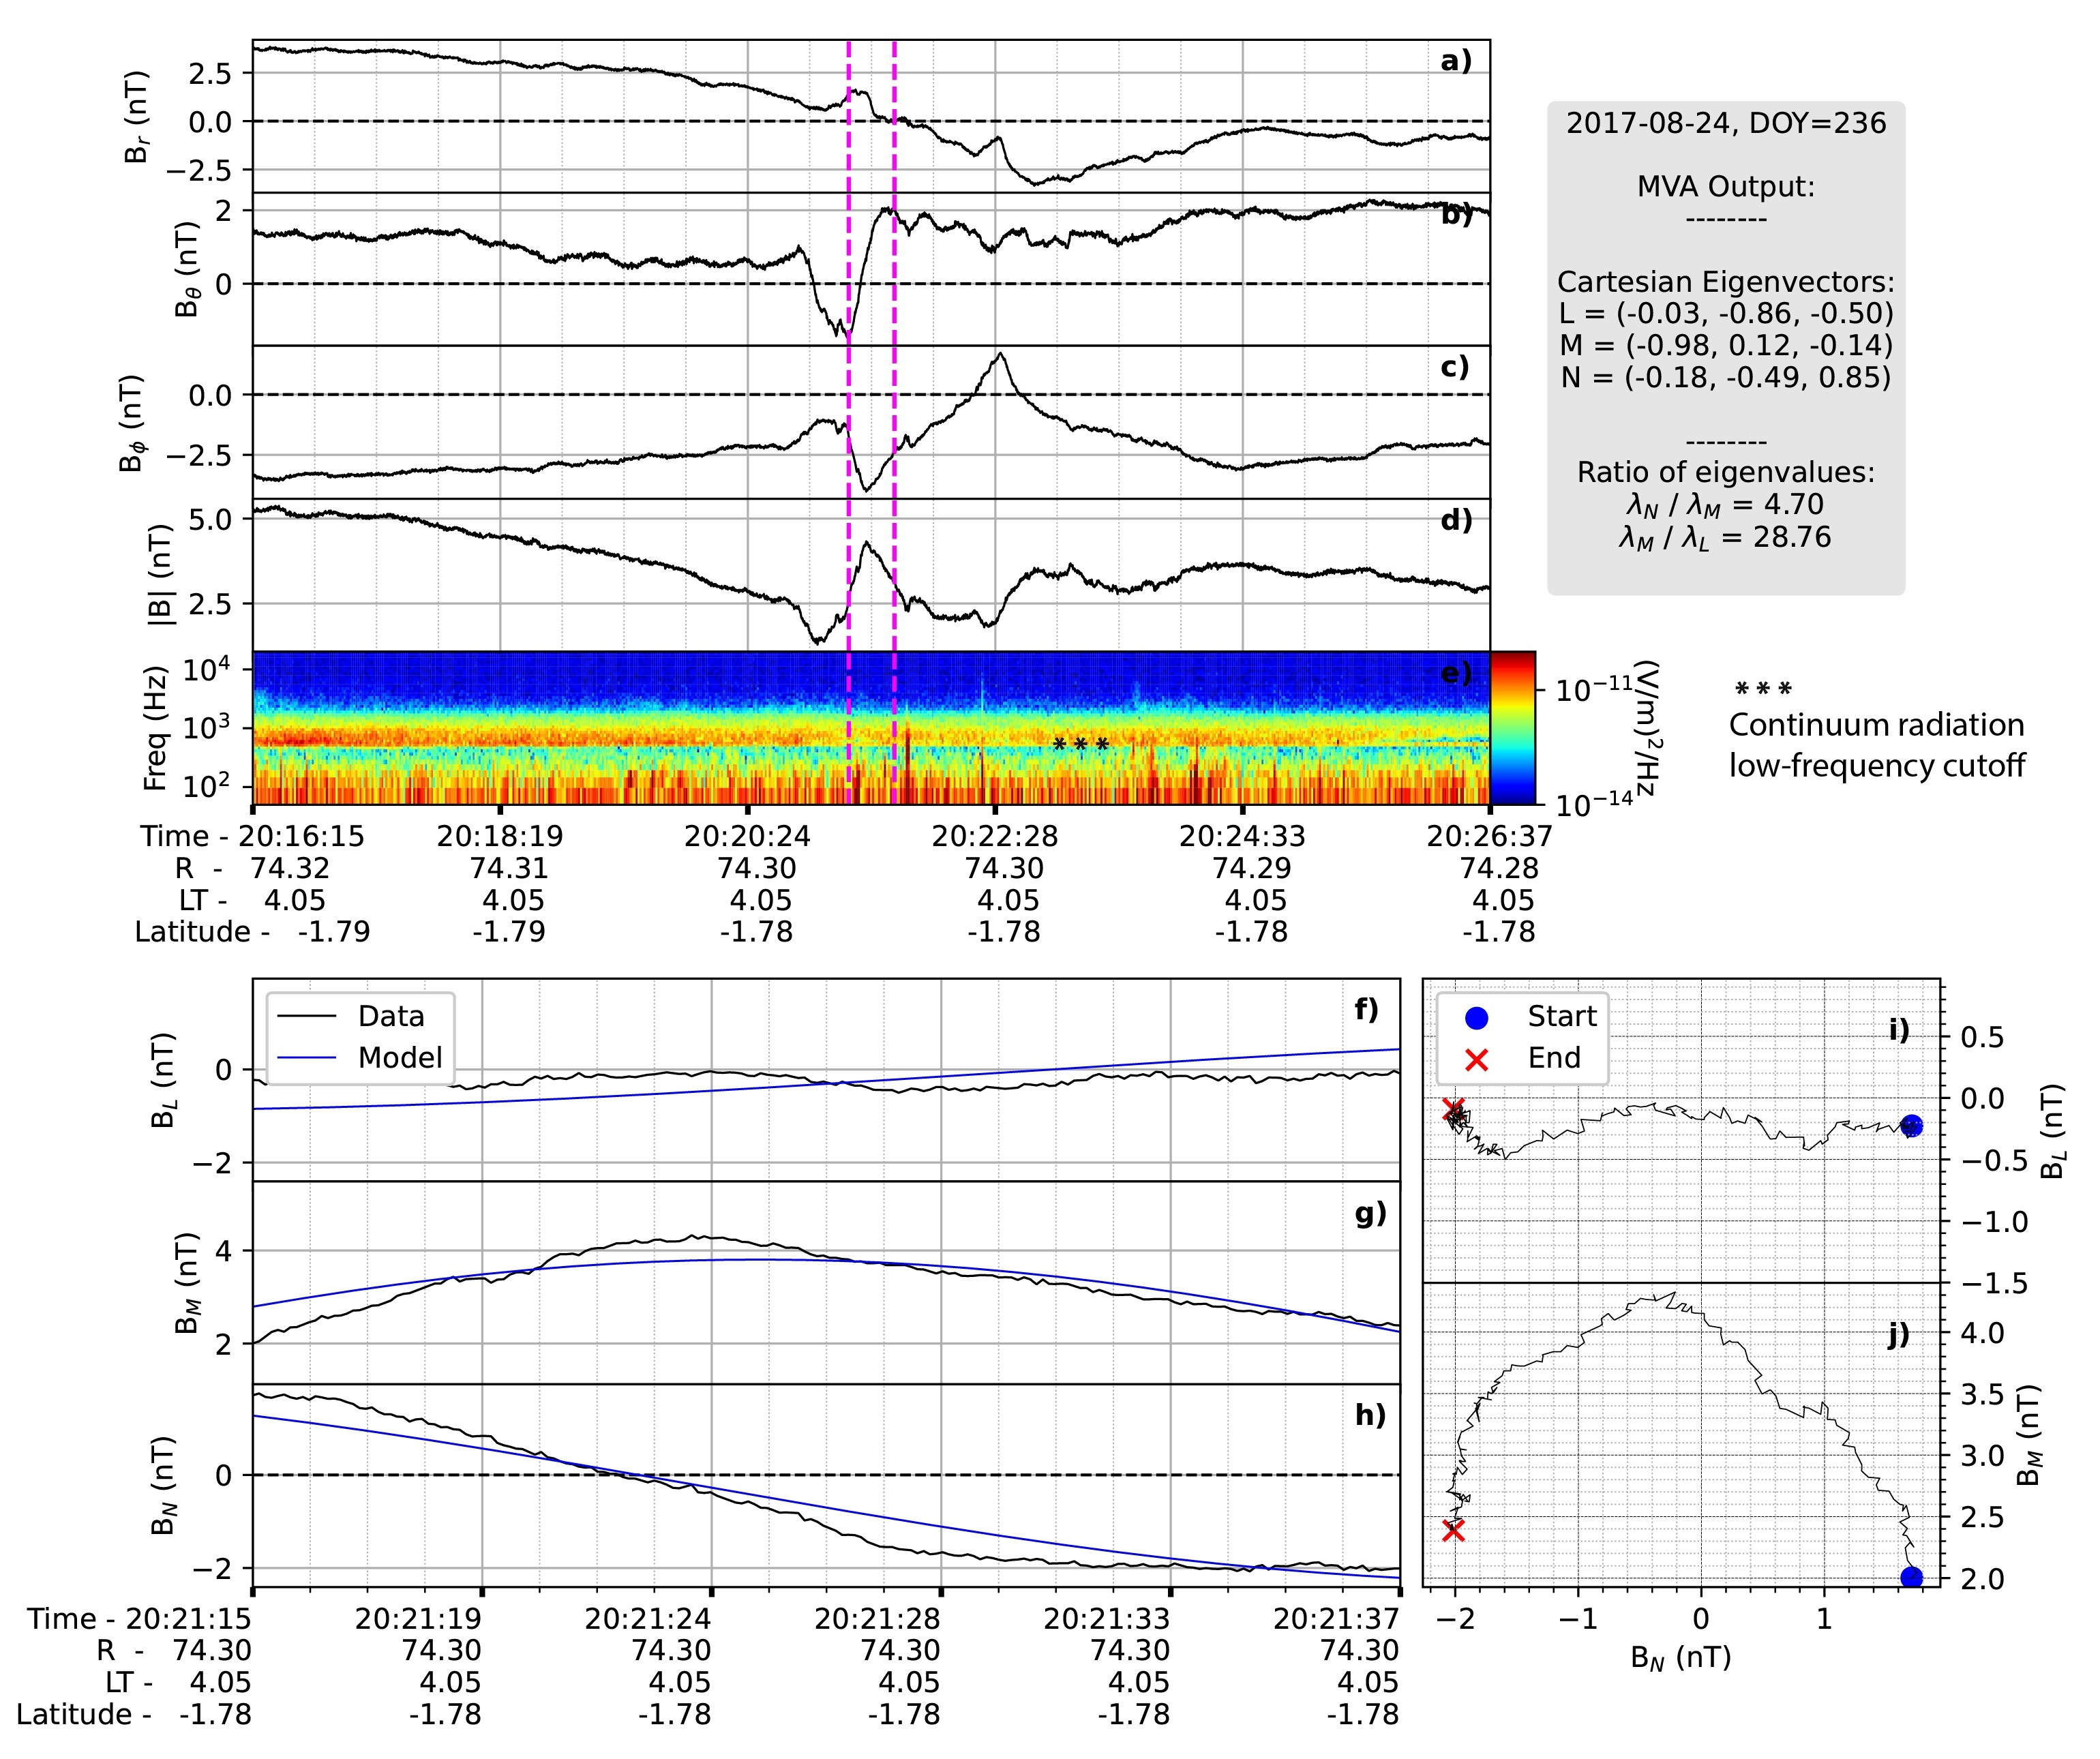
\includegraphics[width=\textwidth]{images5/event-1-fluxrope.jpg}
    \caption{Planetward moving flux rope observed by the Juno spacecraft at DOY 236, 2017. Panels a-d show the magnetic field components in the spherical JSS coordinate system, while Panel e shows the spectra for the electric field measured using the Juno Waves instrument for the given time period. The flux rope structure is highlighted within magenta lines. Panels f-h show the result of the minimum variance analysis and force-free flux rope fitting. Panels i-j are hodograms of the different components obtained using MVA.}
    \label{fig:event-1-fluxrope}
\end{figure}

On DOY 236, 2017 Juno was located 74.3 $R_J$ away from Jupiter at $\sim$ 04 LT (dawnside magnetotail) when it encountered a flux rope between 20:21:15 and 20:21:37 UTC. $B_\theta$ was positive before and after this event, but briefly reversed to negative values during the interval (Figure \ref{fig:event-1-fluxrope}). The positive $B_\theta$ before and after the bipolar signature is consistent with Juno being in the near‐Jupiter plasma sheet where the inward magnetic stress exerted by the stretched, closed magnetic field is balanced by the inward gradient in the plasma pressure. $B_r$ is less than 1 nT during the encounter and $B_\phi$ increases (in the negative) by $\sim$ nT, which is the core field of the flux rope. The difference between the extrema in $B_\theta$ is about 4 nT. The sharp peak in the magnetic field strength, closely aligned with the center of the $B_\theta$ reversal, is a characteristic signature of a flux rope. The flux rope is close to the current sheet, as evidenced by the reversal of $B_r$ from positive‐to‐negative values before and after the event. Although there is both a positive‐to‐negative and negative‐to‐positive polarity reversal of $B_\theta$, the core field peak is seen during the negative‐to‐positive reversal, which hints that the flux rope was traveling planetward.

After performing the MVA, we find a bipolar variation in the $B_N$ (maximum) component and a peak in the $B_M$ (Figure \ref{fig:event-1-fluxrope}), which is expected for a flux rope with a core field. The ratio between the intermediate and minimum eigenvalues of the variance matrix is 4.7, whereas the ratio between the maximum and intermediate values is 28.76. Looking at the $B_M$ - $B_N$ hodograms shown in Figure \ref{fig:event-1-fluxrope}, we can observe a rotation of the magnetic field. Figure \ref{fig:event-1-fluxrope} also shows the magnetic field components of the modeled force‐free flux rope (in blue) in the MVA coordinate system which best fits the data (minimum $\chi_r^2 = 0.13$). The modeled flux rope has a core field strength of 3.86 nT and an impact parameter of 0.0, which indicates that the spacecraft passed very close to the center of the flux rope structure. This is also supported by the extremely low magnitude of $B_L$ (less than 0.4 nT).

The eigenvectors of the variance matrix in the direction of minimum, intermediate, and maximum variance are (in the Cartesian JSS coordinate system) $\mathbf{x}_L=(-0.03,0.86,-0.5)$, $\mathbf{x}_M=(-0.98,0.12,-0.14)$ and $\mathbf{x}_N=(-0.18,-0.49,0.85)$. Although flux ropes in the terrestrial magnetotail typically have a core field in the $Y_\text{JSS}$ direction (as provided by $\mathbf{x}_M$), we find that for this event the direction of intermediate variance is in the $X_\text{JSS}$ direction, which is close to azimuthal direction at the given spacecraft location (Figure \ref{fig:locations-fluxropes-eg}).

\begin{figure}
    \centering
    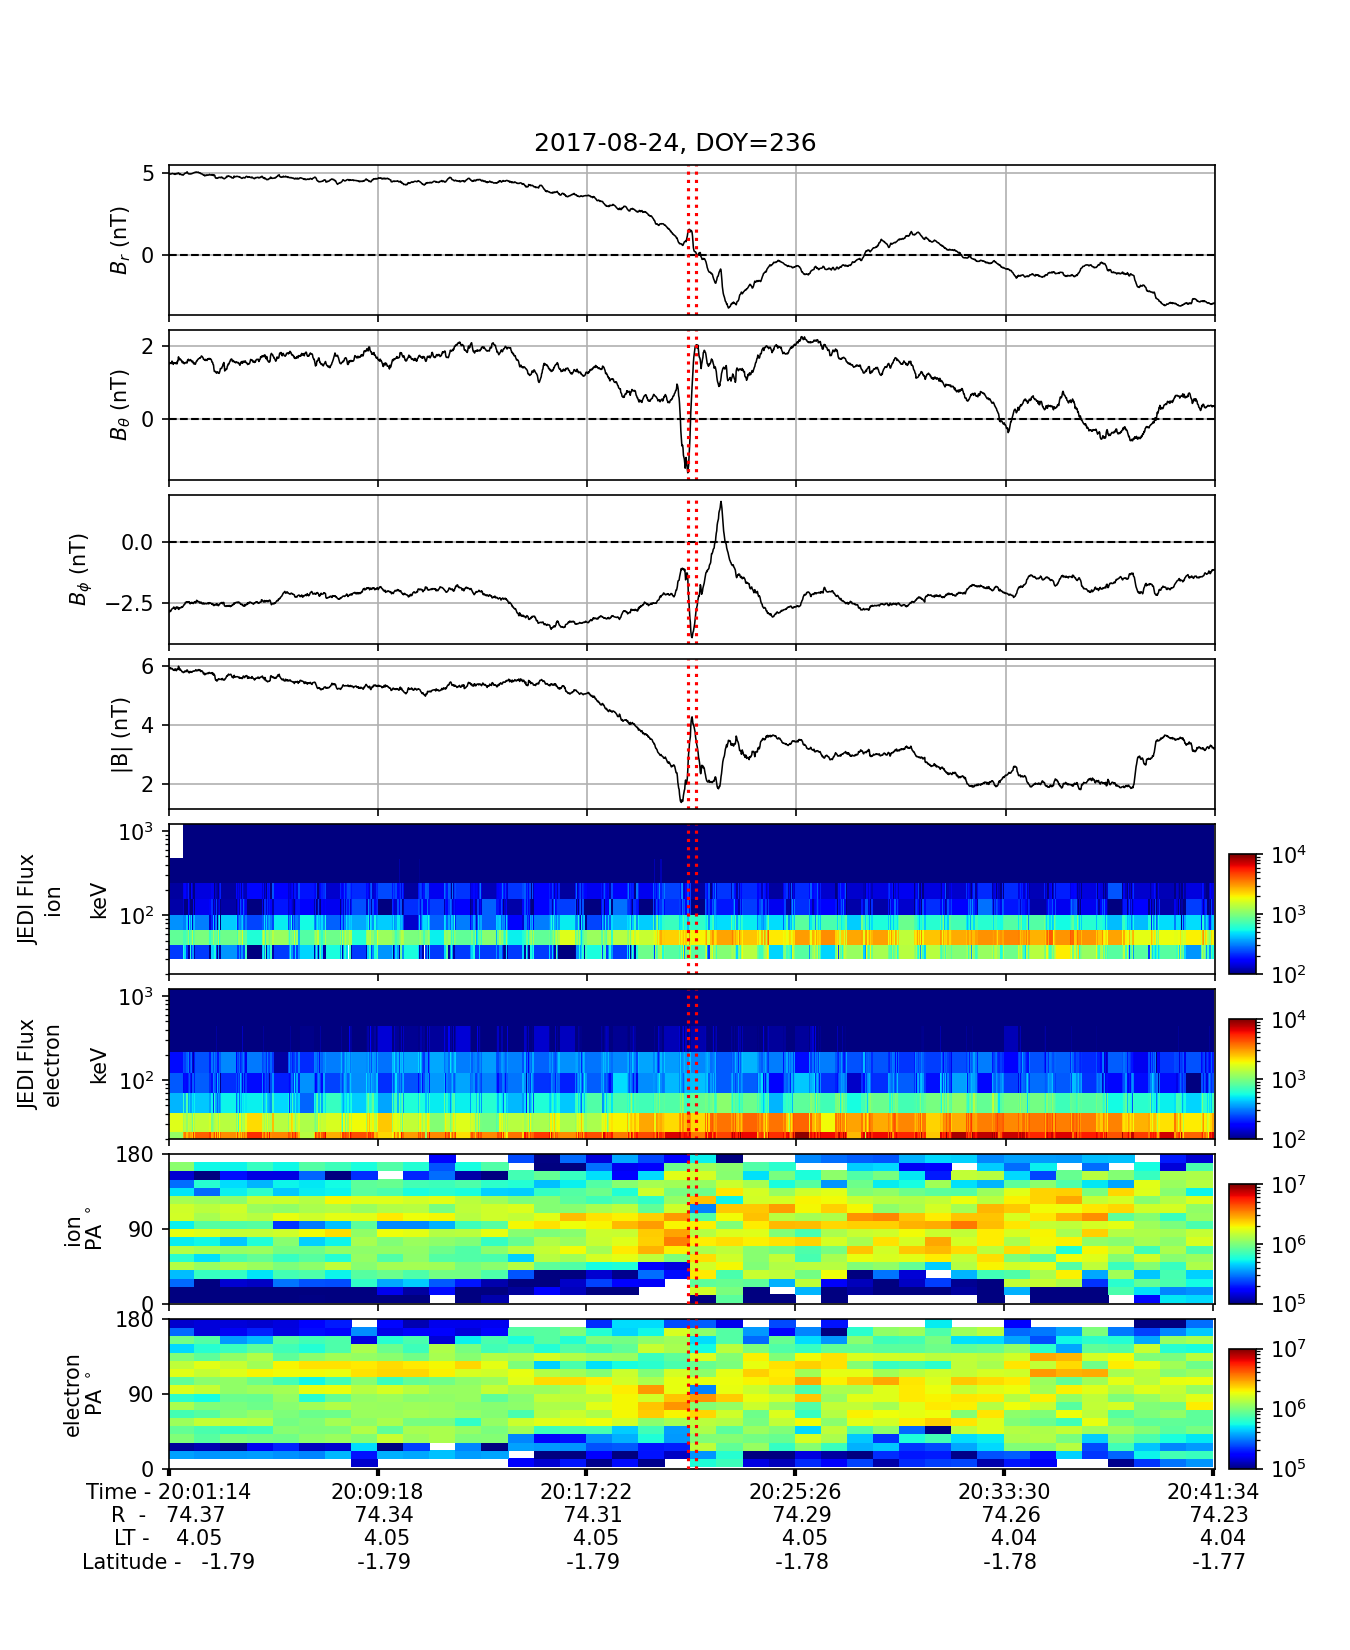
\includegraphics[width=\textwidth]{images5/event-1-jedi.png}
    \caption{The magnetic field observations along with JEDI dynamic spectra for the ions and electrons. The last two rows show the dynamic pitch angle spectra for the protons and electrons respectively.}
    \label{fig:event1-jedi}
\end{figure}

In Figure \ref{fig:event1-jedi}, we show the measurements taken by JEDI in the 40 minute interval centered at the occurrence of Event 1. Panels e and f show the dynamic spectra of the ion and electron flux for all JEDI detectors and Panels g and h show the pitch angle spectra for the protons and the electrons. An increase in the electron and ion flux is seen after the flux rope event, which could be due to the proximity to the equatorial plasma sheet as inferred from the low values of $B_r$. The pitch angle for both ions and electrons is close to 90$^\circ$ prior to the flux rope interval, i.e. both species have a preferential motion in the direction perpendicular to the magnetic field. The anisotropy between parallel and perpendicular flux decreases after the flux rope, with more fluxes in the parallel directions. 


\subsection{Event 2 — Flux Rope DOY 338 2017}

\begin{figure}
    \centering
    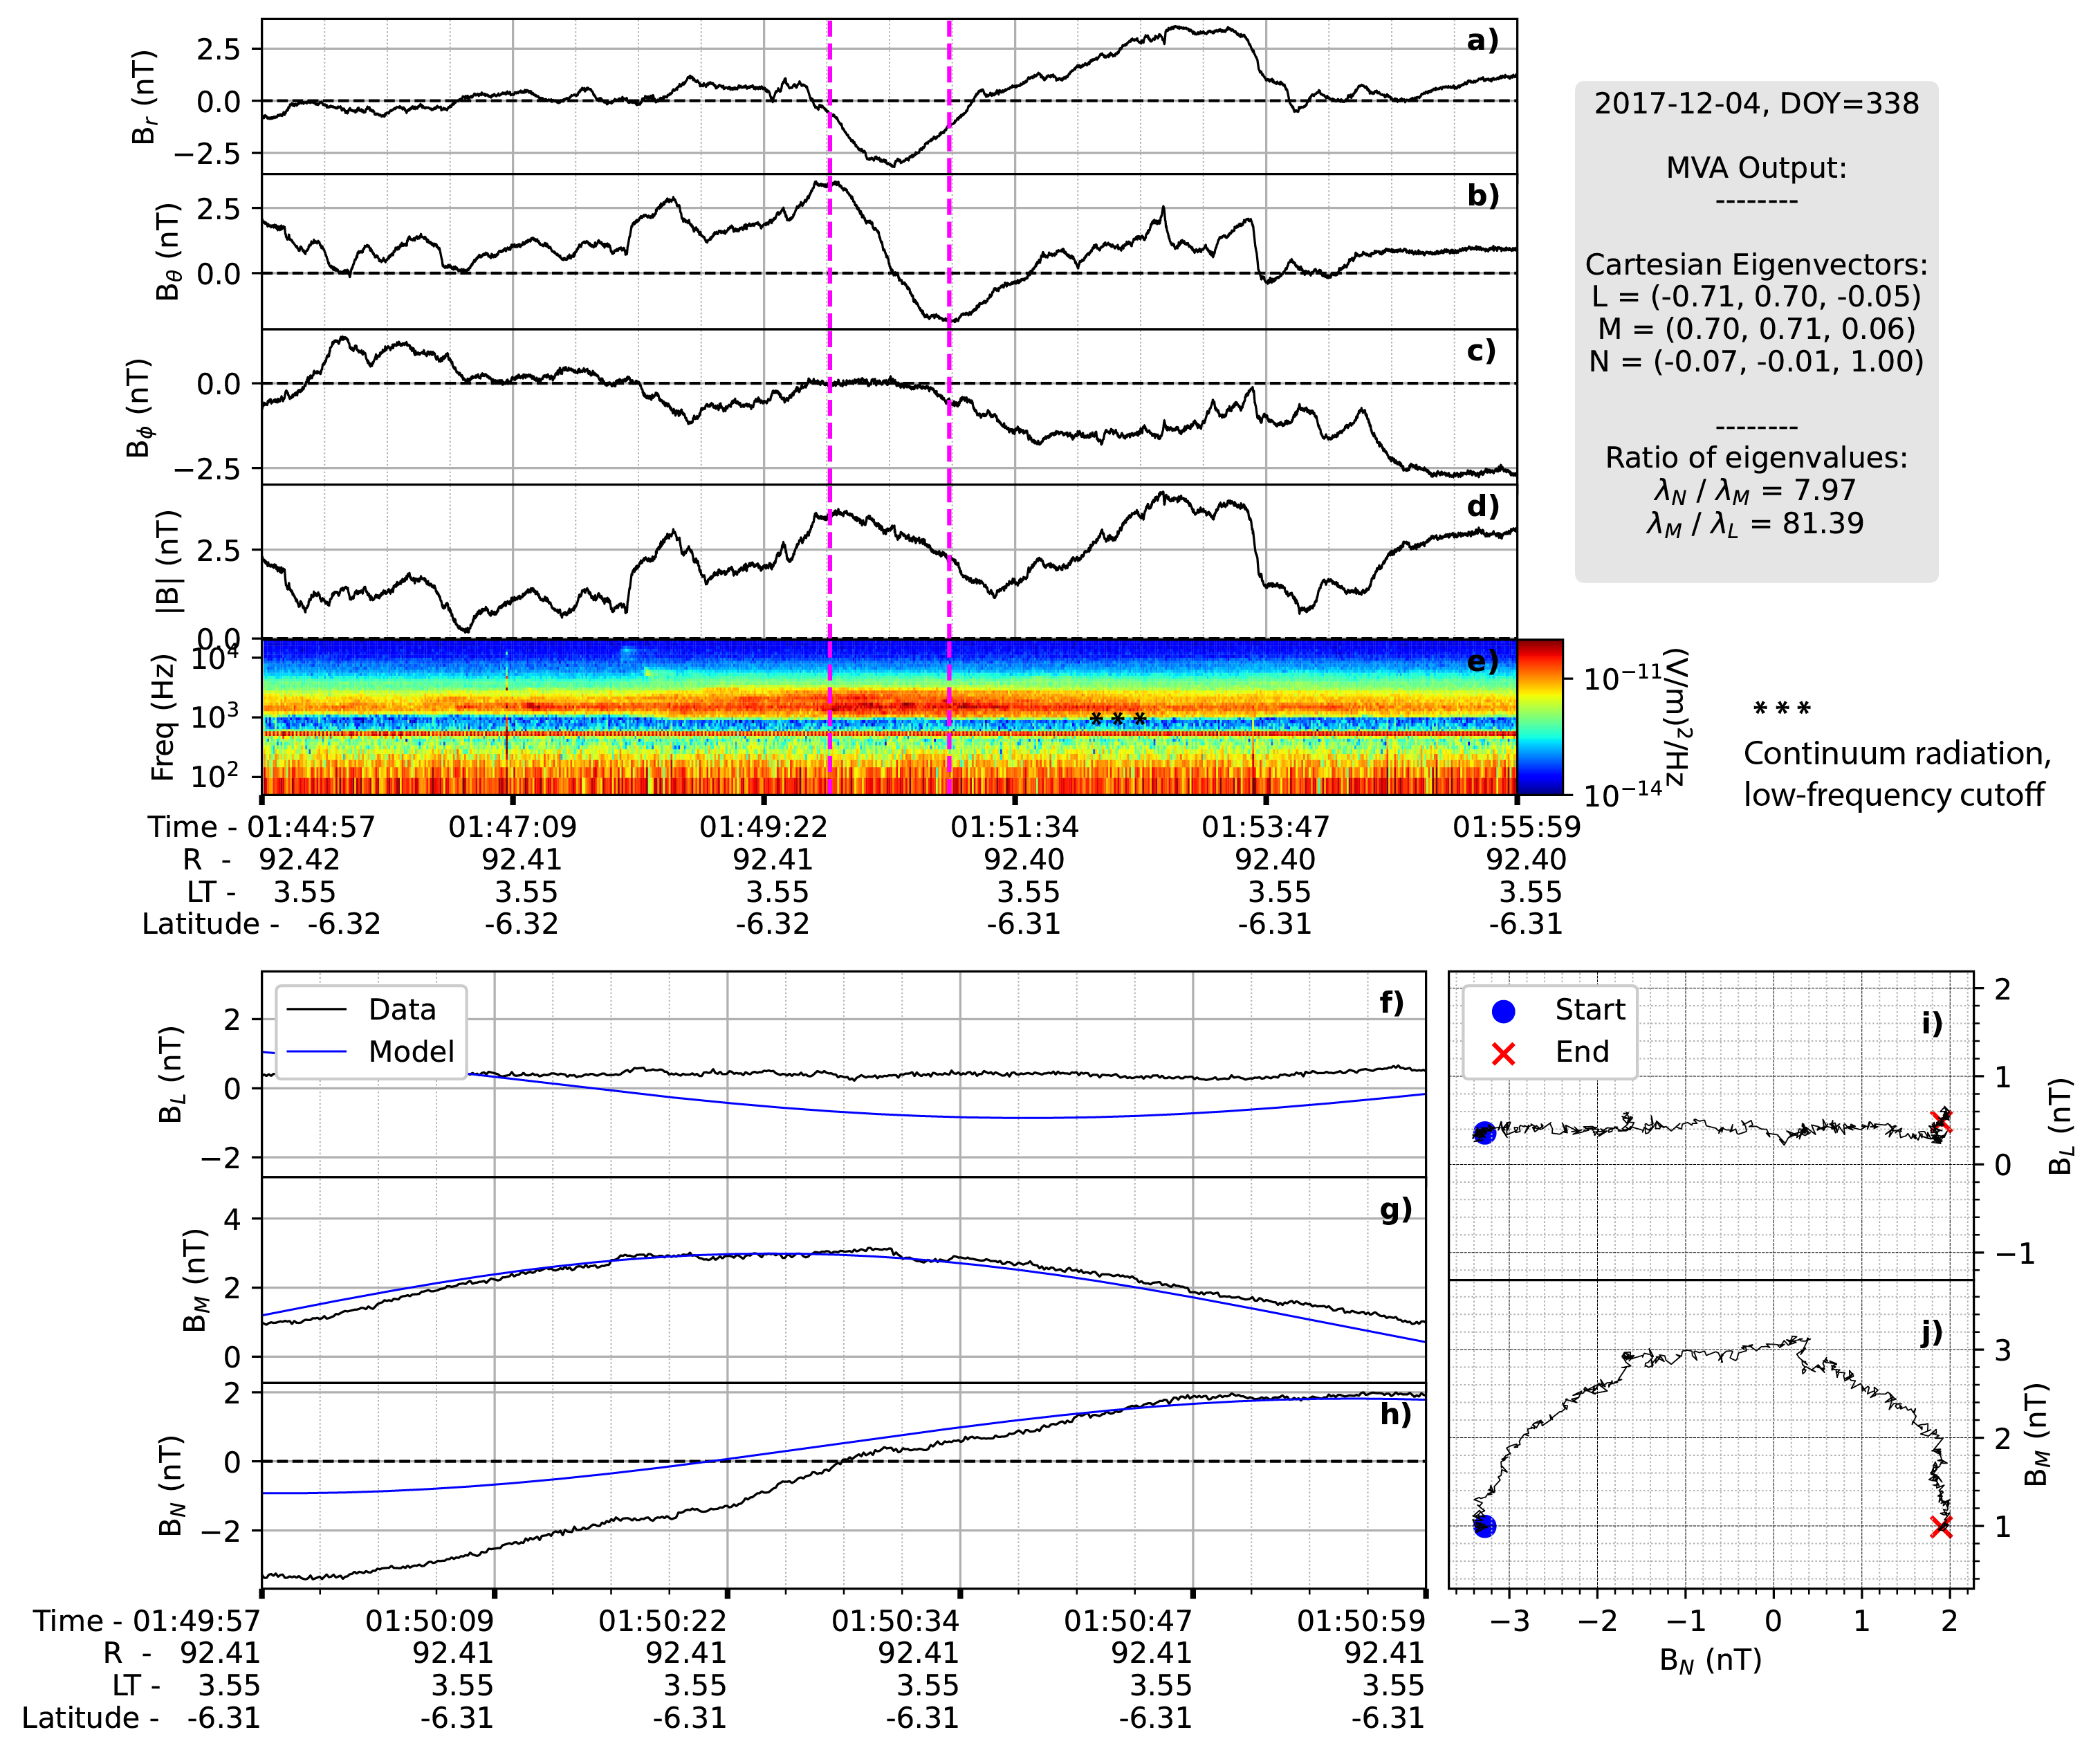
\includegraphics[width=\textwidth]{images5/event-2-fluxrope.jpg}
    \caption{Tailward moving flux rope observed by the Juno spacecraft at DOY 338, 2017. Same format as Figure \ref{fig:event-1-fluxrope}.}
    \label{fig:event-2-fluxrope}
\end{figure}

On DOY 338, 2017 between 01:49:57 and 01:50:59 UTC Juno was located at $\sim$92 $R_J$ between 03 and 04 LT and observed a reversal in $B_\theta$ from positive‐to‐negative values, indicating a tailward moving flux rope (Figures 3a–3d). Unlike the previous example, the magnetic field magnitude did not peak inside the event interval, despite the presence of an axial core field. The azimuthal field component remained close to zero.

Performing the MVA provides us with additional information (Figures 3f–3h)—the maximum variance is in the $Z$ direction ($\mathbf{x}_N=(-0.07,0.01,1.00)$), as expected, whereas the intermediate and minimum variance directions lie in the $XZ$ plane close to the local radial and tangential directions. The component of the magnetic field in the minimum variance direction is close to zero. The intermediate component ($B_M$) peaks in the middle of the event interval. The $B_M$ - $B_N$ hodograms show a clear rotation of the magnetic field.

The spectra for the electric field as observed by the Waves instrument for Event 2 is shown in Figure 3e. A broadband intensification can be seen between 1 and 3 kHz for the duration of this event. Enhanced fluctuations in the electromagnetic field have been seen inside plasmoid intervals in the past in the terrestrial magnetosphere \cite{Kennel1986PlasmaRopes}. Although the continuum radiation is observed during the first event as well, no transient intensification was observed due to the flux rope.

Although Event 1 is an isolated flux rope event during the associated current sheet crossing, that is not true for Event 2. Figure 4 shows the magnetic field observations $\sim$2 h before and after Event 2. Multiple, alternating $B_\theta$ reversals, with peak‐to‐peak durations of roughly 2-3 min or more were observed prior to the event, and the continuum radiation can be seen throughout the $\sim$2 h current sheet crossing interval. For context, during the same day (DOY 338, 2017), \citeA{Vogt2020MagnetotailObservations} also report two large events observed at times 4:15 and 17:47 UTC.

Data from the JEDI instrument for this interval is sparse and cannot be used for further analysis.

\subsection{Case studies - Discussion}

The duration of the two events discussed in this study, as defined by the time between extrema in $B_\theta$, is roughly 22 and 62 s, respectively. Using the low-frequency cutoff for the continuum radiation, which is roughly between 500 and 600 Hz for Event 1 and $\sim$1 kHz for Event 2, we estimate the plasma densities \cite{Barnhart2009ElectronSpectra} during the intervals in question to be 0.003 and 0.012 cm$^{-3}$, respectively, which correspond to ion inertial lengths of roughly 16356 (0.23 $R_J$) and 8178 km (0.11 $R_J$), assuming an ion mass of 16 amu. Assuming that the plasmoid travel speed is limited by the Alfven speed in the surrounding lobes \cite{Cowley2015Down-tailMagnetospheres} which are 489 and 220 km/s (which is calculated based on the observed magnetic field strength of 5 and 4.5 nT, respectively and electron density obtained from Waves), the 22 and 62 s duration of the event would correspond to diameters of roughly 10771 km (0.15 $R_J$ or 0.65 $d_i$) and 13360 km (0.19 $R_J$ or 1.67 $d_i$), respectively. \citeA{Kronberg2008MassParameters} found that most energetic particle bursts corresponding to plasmoid events have speeds of roughly 450 km/s, which would provide diameters of 9900 km (0.6 $d_i$) and 27900 km (3.4 $d_i$) for the two events respectively, comparable to the local ion inertial length.

After Event 1, when the flux rope has passed over the spacecraft, a reversal in the guide field ($B_\phi$) is observed from -4 to 2 nT. This reversal of the out‐of‐plane component of the magnetic field in close proximity to the reconnection x‐line could be due to the quadrupolar Hall magnetic field \cite{Eastwood2007Multi-pointOn,Sonnerup1967MagnetopauseObservations}, which is formed due to the decoupling of ions and electrons in the ion diffusion region and has been identified by multiple spacecraft in the terrestrial magnetotail \cite{Nagai2001GeotailMagnetotail}. We caution however that single‐spacecraft measurements are unreliable to conclusively determine whether or not the reversal in $B_\phi$ is due to the Hall field. Another possible explanation for the reversal could be related to the bend-back of the magnetic field, which has been seen as a correlation between the sign of $B_r$ and $B_\phi$. In the present situation, the latter theory is less likely since $B_\phi$ returns to negative values despite multiple current sheet crossings as seen in $B_r$.

For Event 2, the MVA analysis shows that Juno is sampling the portion of the flux rope where its axis is almost radial, as determined by the direction of intermediate variance. The ratio of the maximum to intermediate and intermediate to minimum eigenvalues are quite large ($\lambda_N/\lambda_M =7.97$, $\lambda_M/\lambda_L=81.31$), indicating that the coordinate system is well‐defined. Note that observations of flux ropes in the terrestrial magnetotail have shown that many flux ropes are tilted in the plane of the current sheet \cite{Slavin2003GeotailSheet}. However, $|\mathbf{B}|$ does not peak at the center of the interval and the best fit force‐free flux rope does not fit the data well ($\chi_r^2 = 5.9$), although the modeled field in the $B_M$ component looks reasonable, and a bipolar signature is observed in the $B_N$ component. While conventionally flux ropes in the terrestrial magnetotail are seen to possess a strong core field, this has not been the case for the giant planet magnetospheres. Plasmoids observed at Jupiter and Saturn usually possess a weak magnetic field at their core, which is likely due to large plasma $\beta$. The force‐free model is based on the assumption that pressure gradients inside and surrounding the flux rope are negligible, which may not be the case for this event. Another possible explanation is that this is a flux rope in the early stages of formation and has not yet reached the minimum energy force‐free state.

\begin{figure}
    \centering
    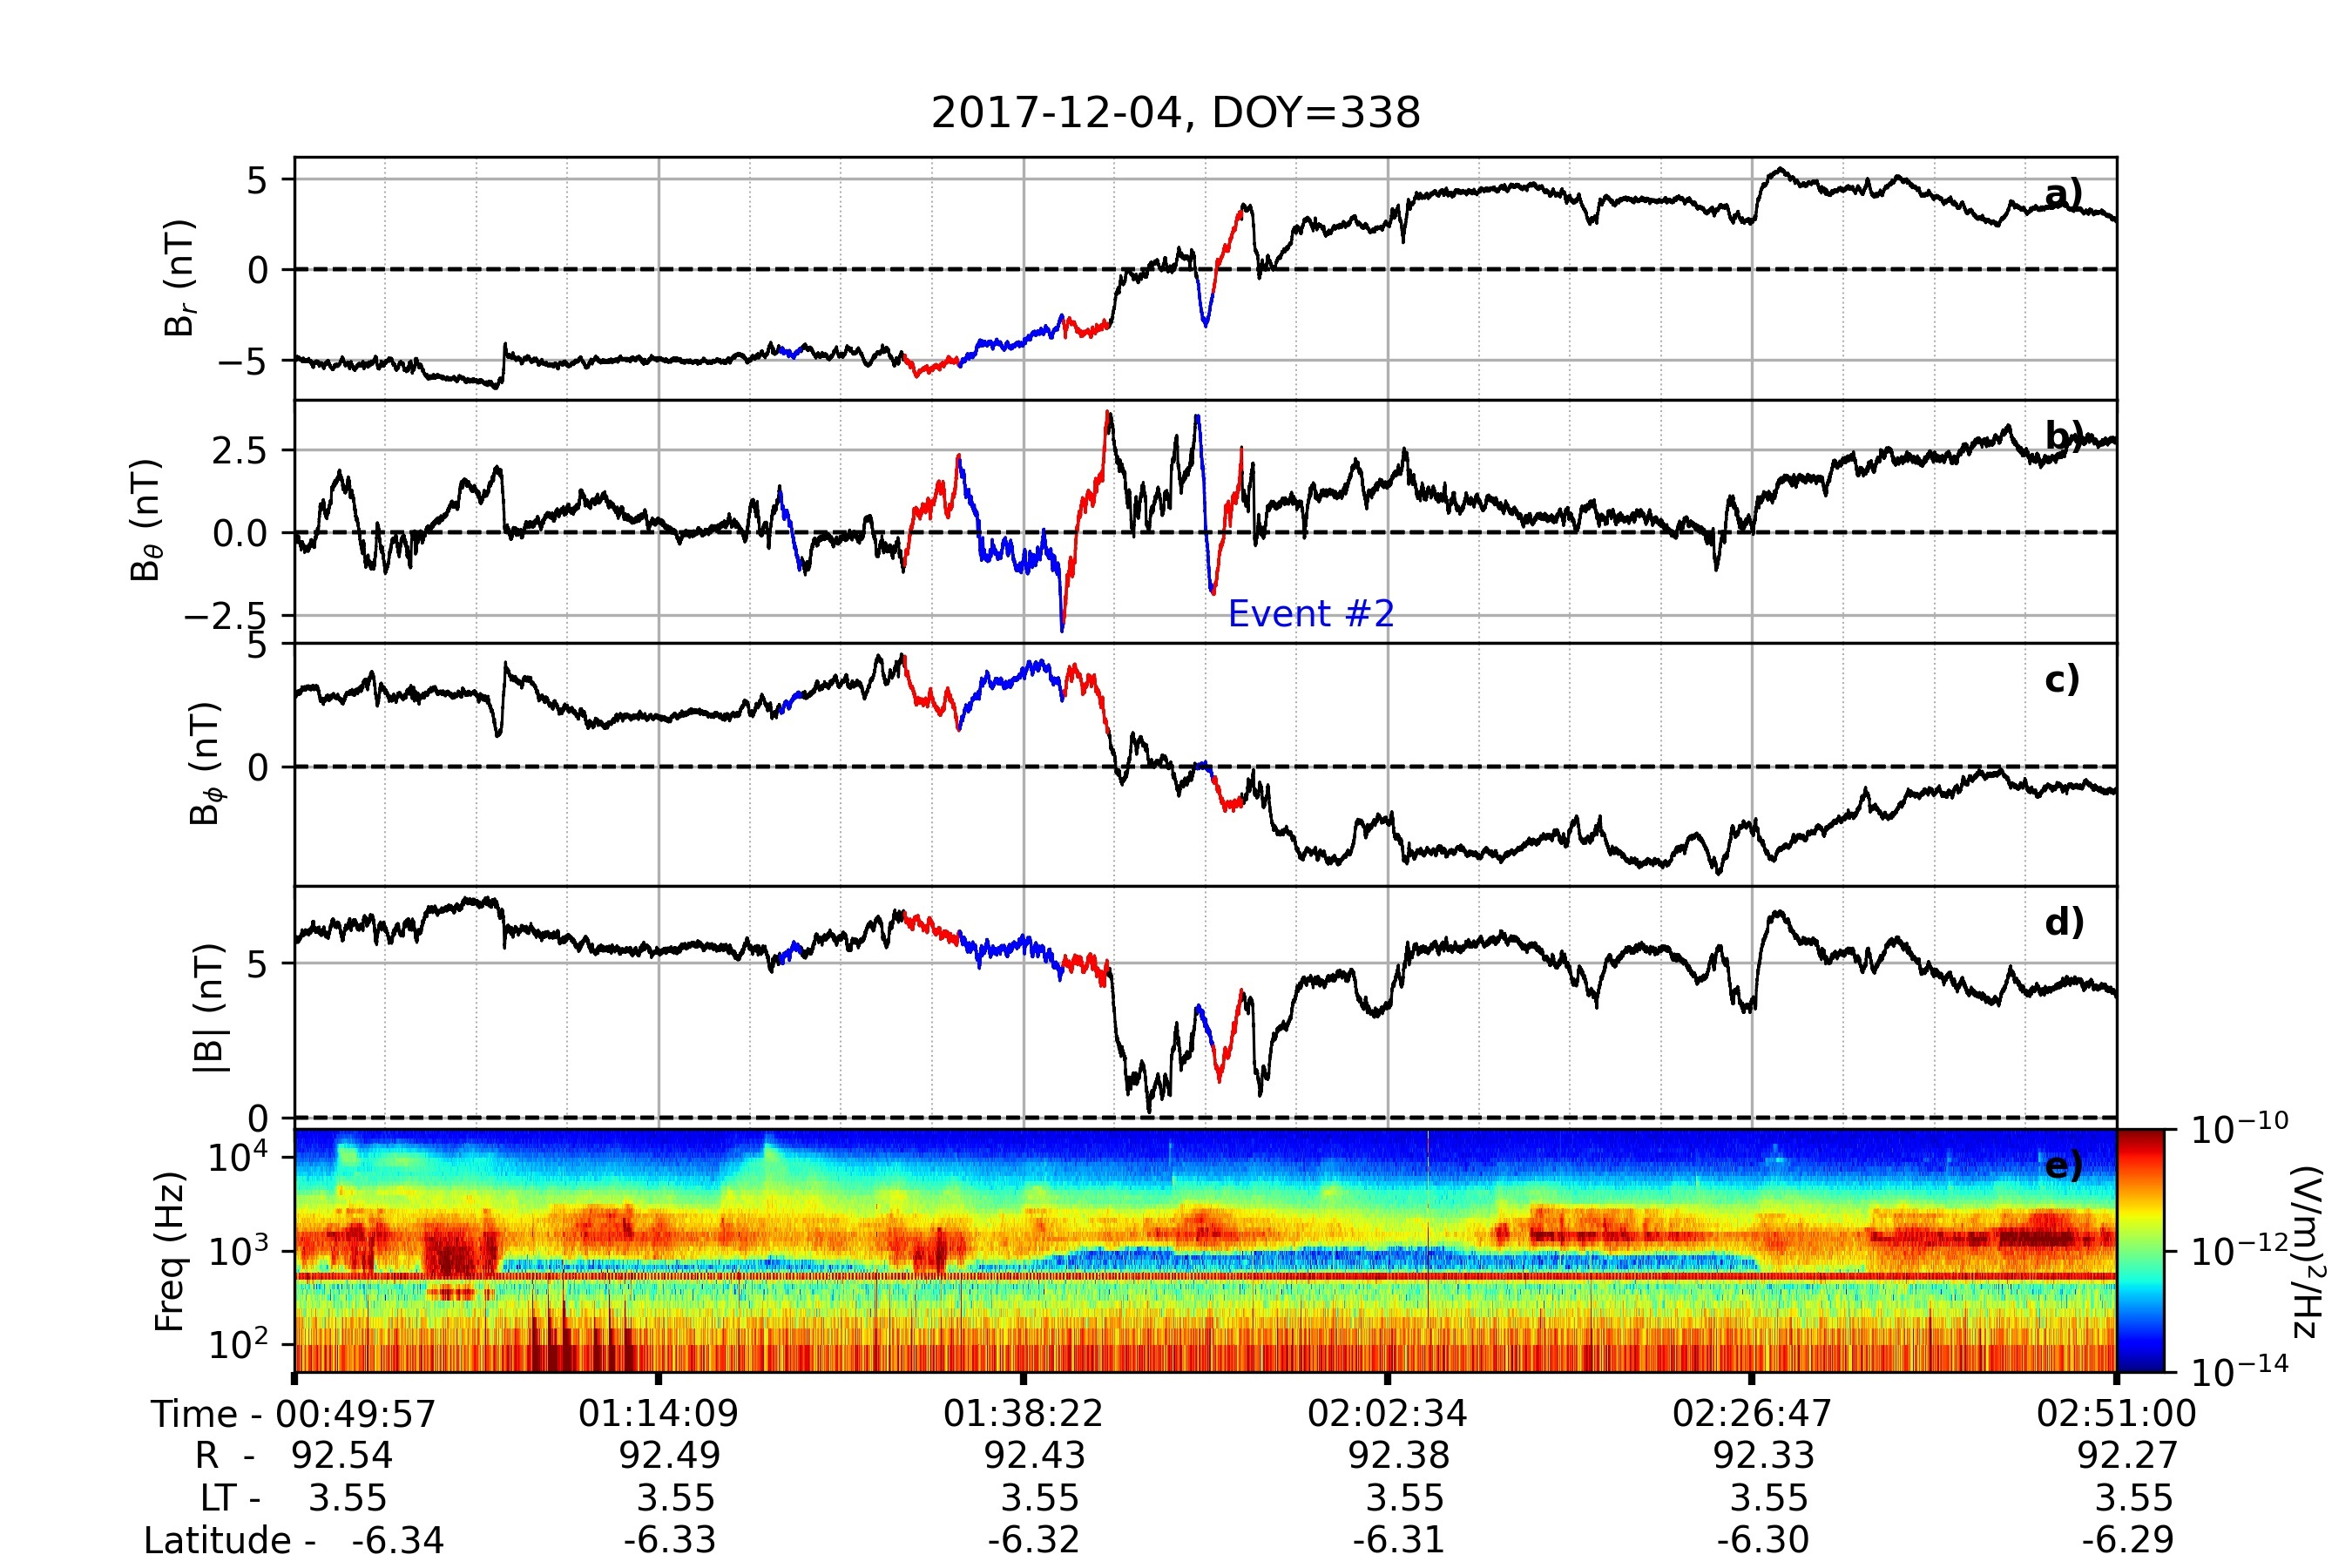
\includegraphics[width=\textwidth]{images5/event-2-context.jpg}
    \caption{Caption}
    \label{fig:event-2-context}
\end{figure}

Multiple alternating $B_\theta$ reversals, with peak‐to‐peak durations of roughly 2-3 min or more were observed prior to Event 2 (\ref{fig:event-2-context}, shown in red and blue). There is no clear increase in the axial magnetic field strength inside these events, which indicates that these north‐south reversals correspond to magnetic O-lines. These observations of recurring north‐south reversals are similar to those expected for sequentially released plasmoids from a reconnection X-line due to current sheet instabilities, though single-point measurements are not definitive.

Both events are observed in the dawnside magnetotail, where plasma density is relatively low and the Dungey‐cycle flux closure is expected to occur \cite{Cowley2003b}. However, without context of the global magnetosphere, it is not possible to determine whether the reconnection events discussed here were a product of the Dungey or Vasyliunas cycles. Note that both Dungey and Vasyliunas cycle plasmoid release can be initiated by reconnection initially within closed field lines, as proposed by theoretical models \cite{Cowley2008} and seen in global simulations \cite{Sarkango2019}.

\section{Results - Survey of flux ropes and O-lines}

\subsection{Duration and scale of plasmoid events}

\begin{figure}
    \centering
    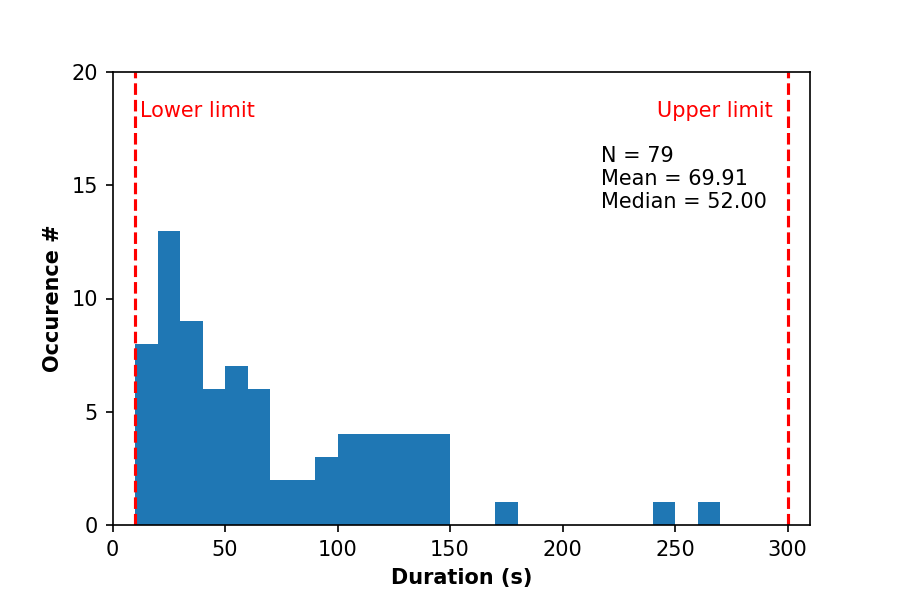
\includegraphics{images5/duration_histogram.png}
    \caption{Caption}
    \label{fig:duration-histogram}
\end{figure}

\begin{figure}
    \centering
    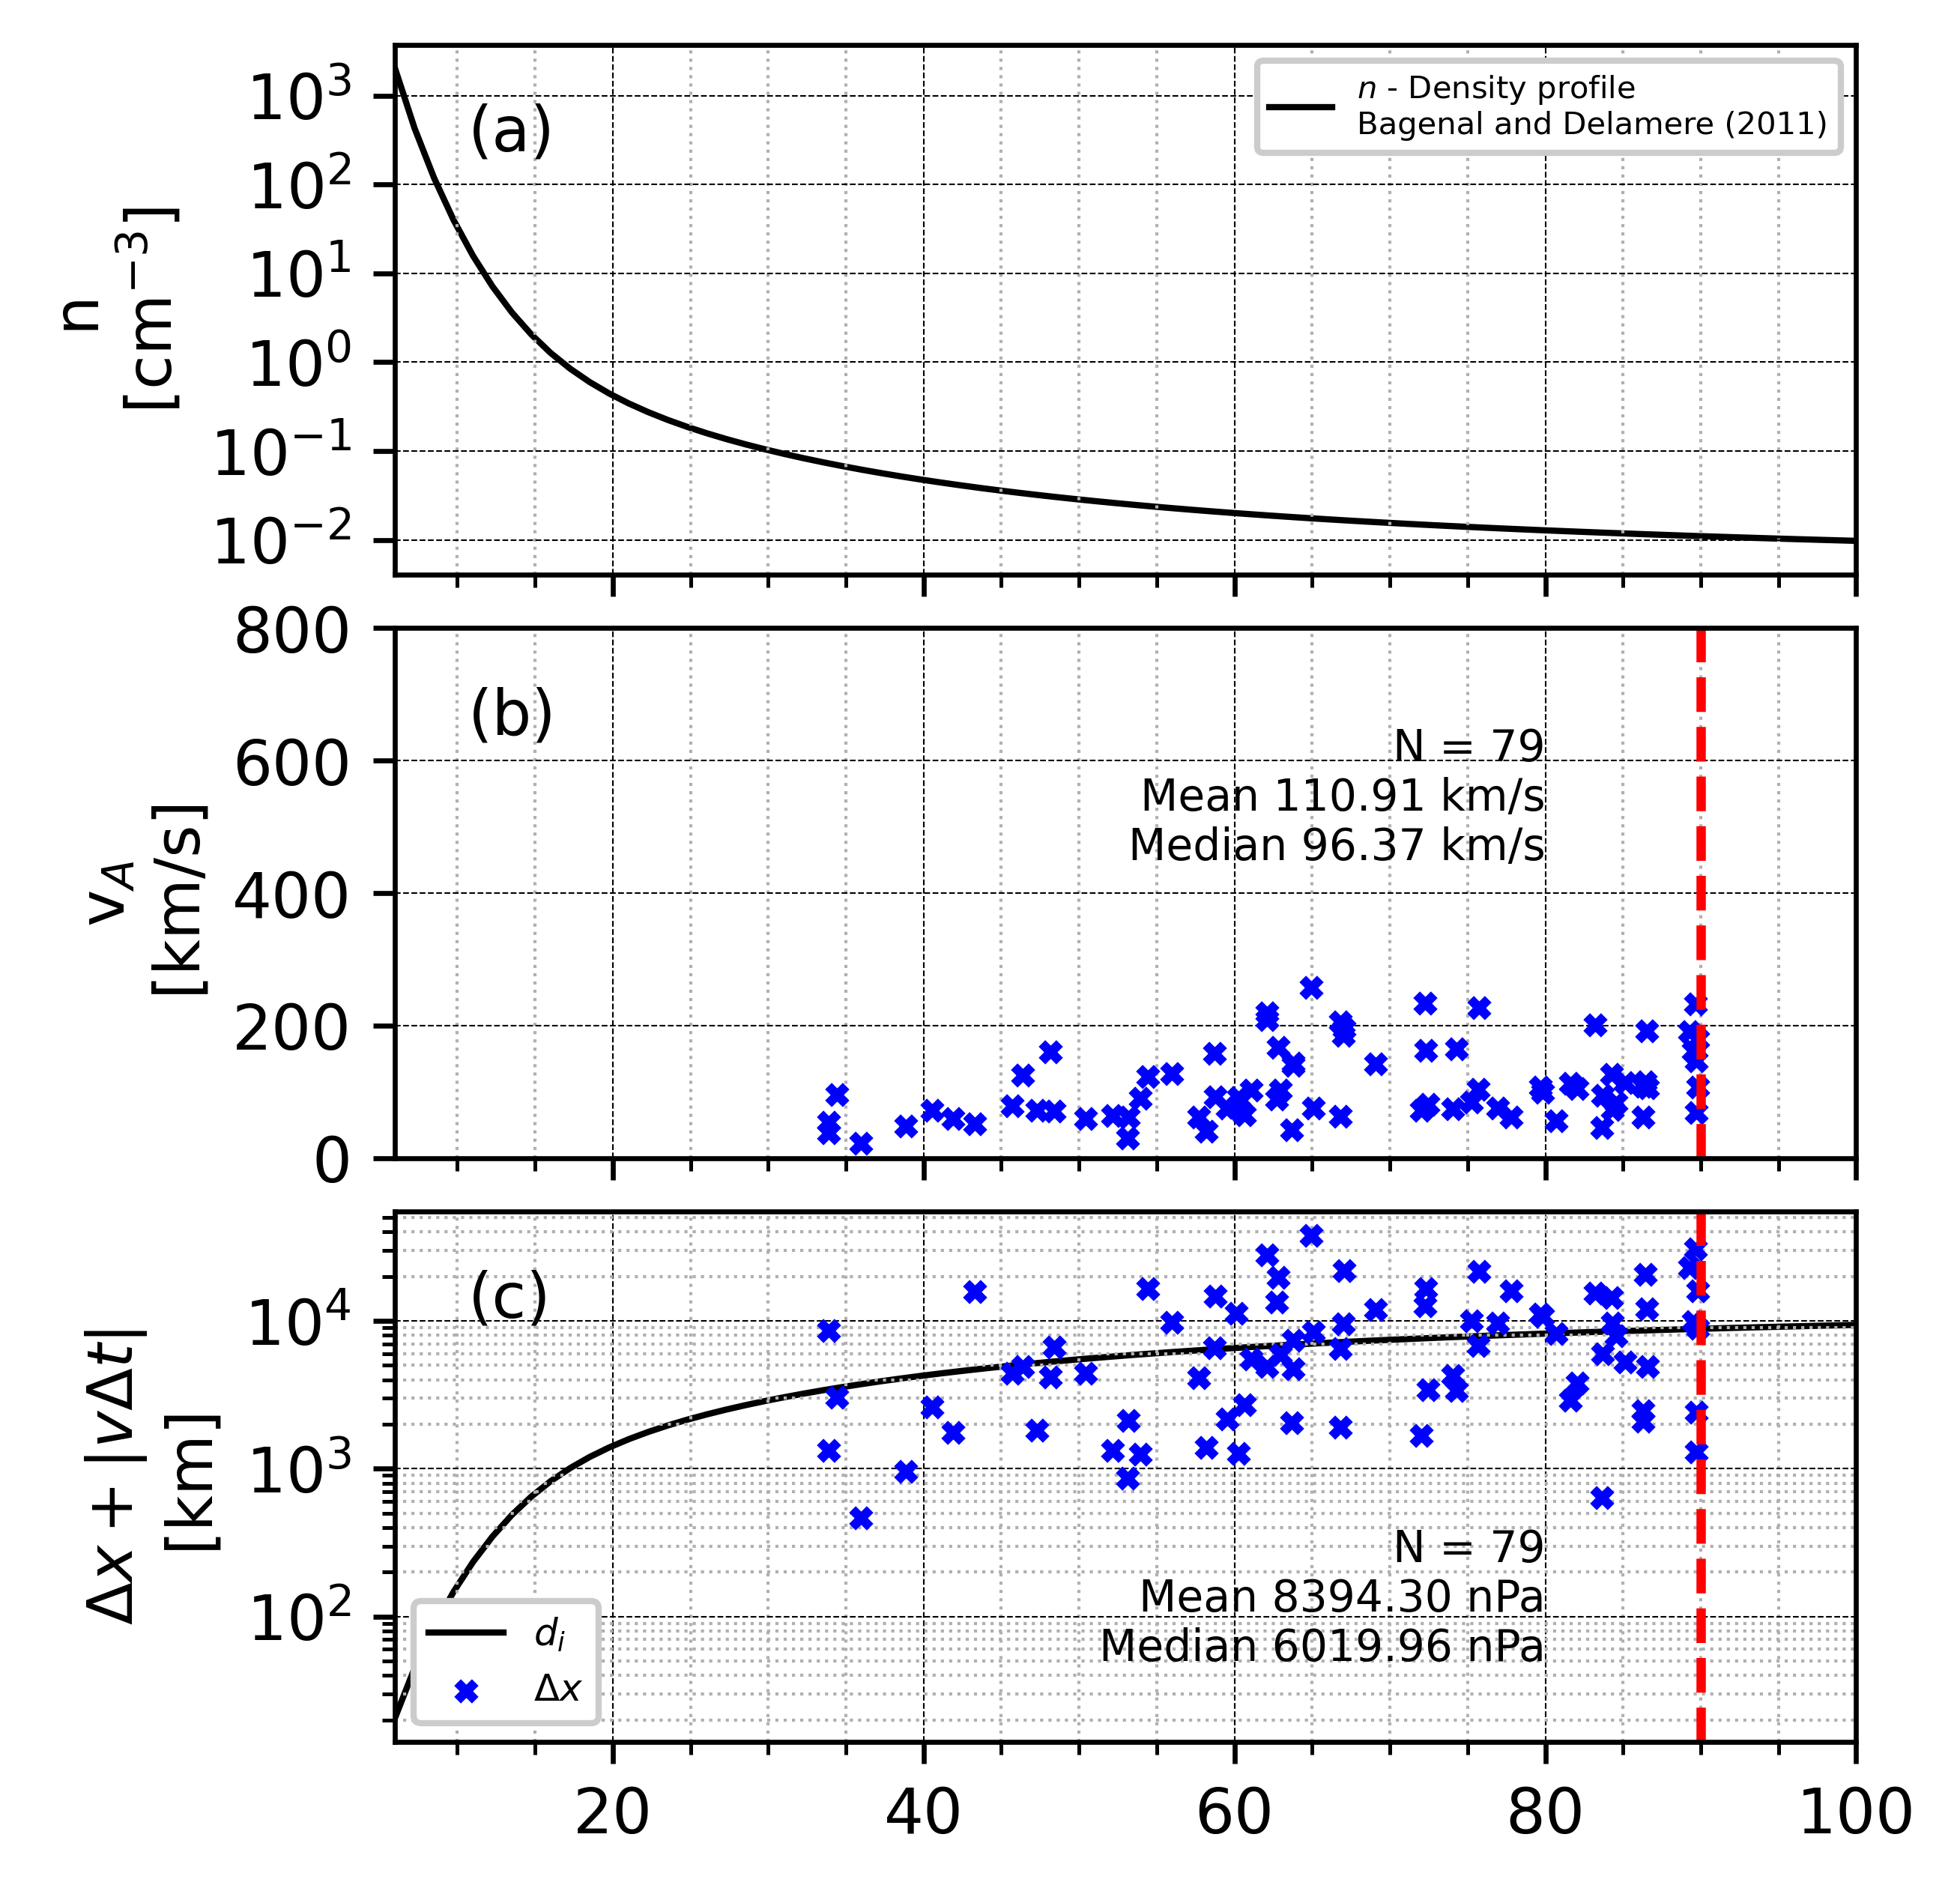
\includegraphics[width=\textwidth]{images5/ion_inertial_selected.png}
    \caption{Caption}
    \label{fig:ion-inertial-scale}
\end{figure}

\begin{figure}
    \centering
    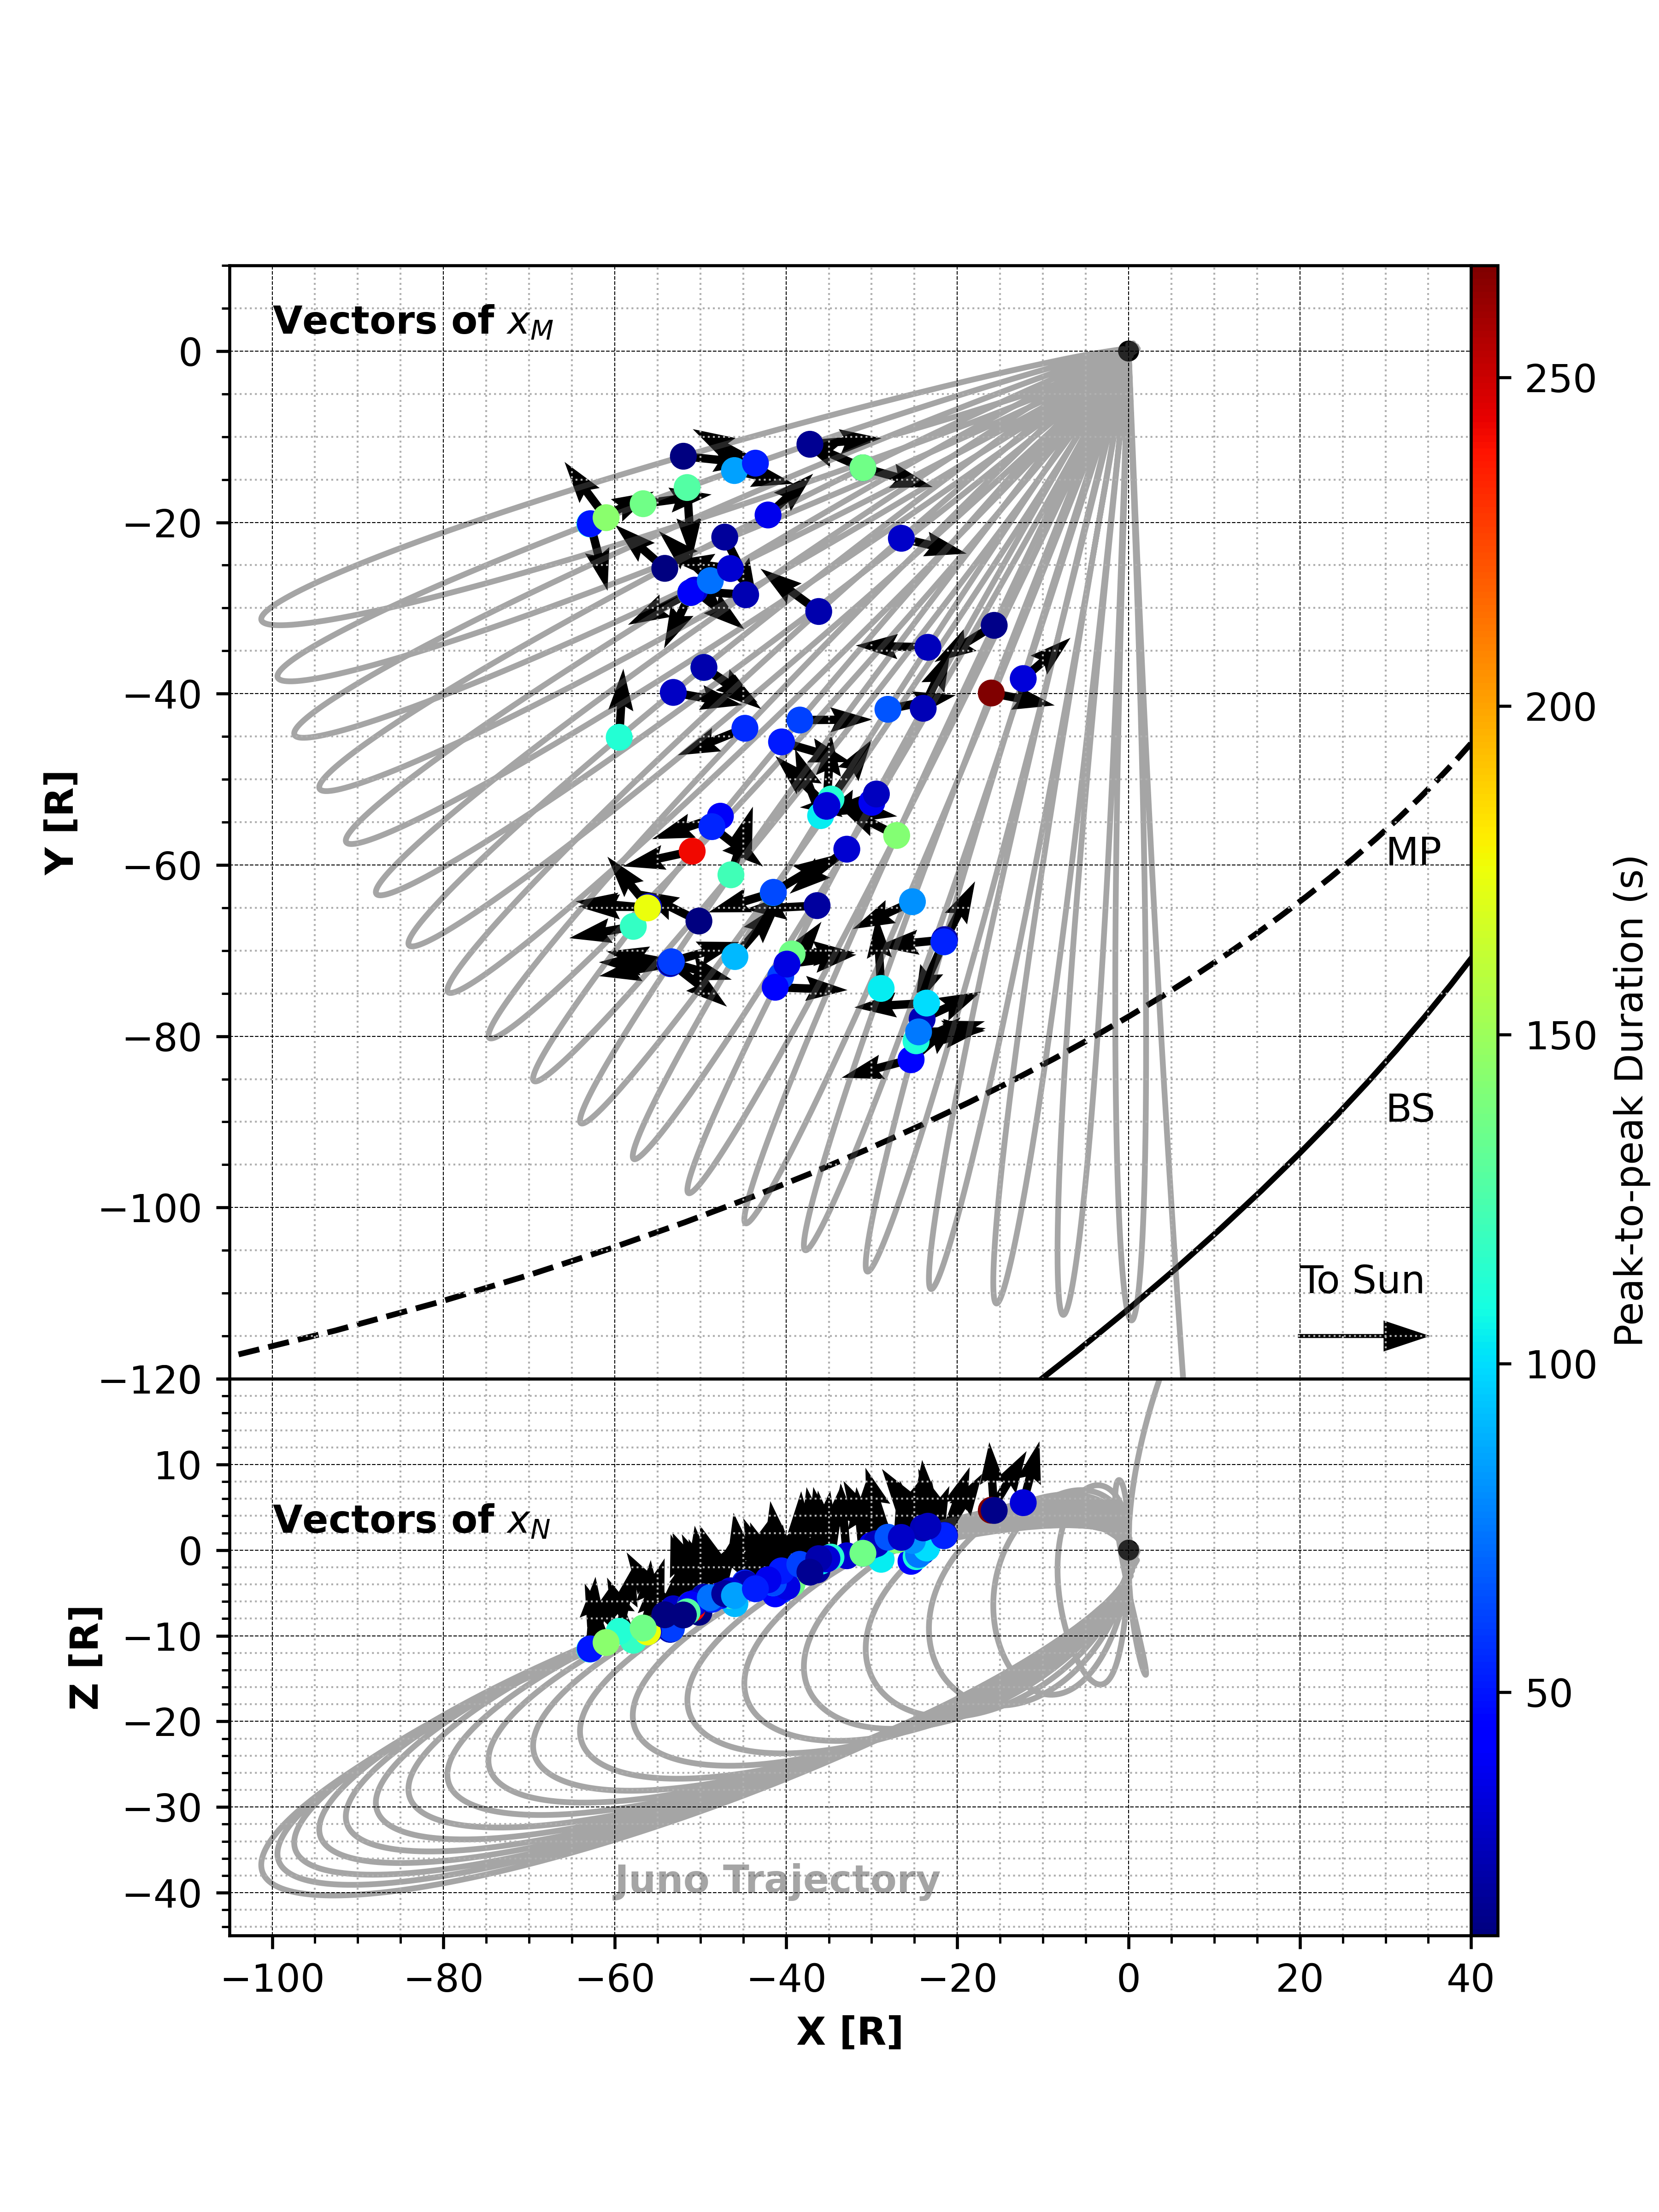
\includegraphics{images5/TrajectoryLocationofEvent_quiver_selected.png}
    \caption{Caption}
    \label{fig:trajectory-quiver}
\end{figure}

\subsection{Flux ropes versus O-lines}

\subsection{Discussion - Survey}

\section{Summary}

Despite differences in magnetospheric dynamics, reconnection occurs in the Jovian magnetotail and releases plasmoids, much like at Earth and Mercury. However, unlike at the terrestrial‐like planets, where plasmoids (or O‐lines) and flux ropes are observed in various sizes, with some at or below the ion inertial length, Jovian plasmoids and flux ropes were observed to be fairly large, with diameters of several $R_J$ (or an order of magnitude larger than the local ion inertial length) or an in situ magnetic signature that is seen to last 6 min on average \cite{Vogt2014}. Potential ion‐scale structures, however, could not have been detected by the Galileo magnetometer, owing to its low temporal resolution of several seconds per vector.

In this letter, we report on observations made by the Juno spacecraft of two magnetic flux ropes in the Jovian magnetotail, whose diameters are comparable to the local ion inertial length. Similar to previous studies, the two events were selected based on a bipolar variation in urn:x-wiley:00948276:media:grl61746:grl61746-math-0054, the component of the magnetic field normal to the current sheet. Each event was further analyzed using the MVA to infer the orientation of the flux rope and modeled using a constant urn:x-wiley:00948276:media:grl61746:grl61746-math-0055 force‐free model. Also seen preceding one of the events are multiple reversals in the north‐south component of the magnetic field, which could be a result of sequential plasmoid release from multiple X‐line reconnection.

While the large‐scale dynamics of the Jovian magnetosphere may be determined by the relatively large plasmoids reported by earlier investigations, the observations reported in this letter show that ion‐scale flux ropes also exist in the Jovian magnetotail, much like at Earth and Mercury. How these flux ropes influence the mass and energy budget of the magnetosphere remains an open question, for which additional surveys are needed to understand their distribution, size, mass, and frequency of occurrence. Moreover, the dusk‐side magnetotail has not been explored in detail, either by Galileo or Juno. An understanding of reconnection, or lack thereof, in this region is crucial to understand how Iogenic plasma ultimately escapes the Jovian magnetosphere.
